\chapter{Provably Robust Skipping-based Probabilistic Data Structures}

In this chapter we consider a distinct subset of probabilistic data structures, which ensures correctness (and hence are not compressing) while offering fast probabilistic runtime guarantees, have received considerably less attention in the literature. Existing security analyses, such as those addressing the robustness of hash tables \cite{CrosbyW03, aumasson2012hash, bar2007remote, eckhoff2009hash,klink2011efficient,bottinelli2025hash} and skip lists \cite{nussbaum2019skiplist}, provide valuable insights but lack formal adversarial models and rigorous security analyses. Due to their runtime properties, we refer to these as \emph {probabilistic skipping-based data structures} (PSDS), as they inherently ``skip'' over parts of their internal structure to accelerate lookup operations.
The lack of research in this area is particularly concerning given that the studies on hash tables have already uncovered practical attacks, including methods to mount denial-of-service attacks attacks against intrusion detection systems~\cite{bar2007remote}, web application servers \cite{klink2011efficient}, and the QUIC protocol~\cite{bottinelli2025hash}.


%-------------------------------------------------------------------------------
\section{Relation to Previous Work}
\subsection{Self-Balancing and Self-Organizing Data Structures}

Although PSDS share conceptual similarities with self-balancing and self-organizing data structures, they differ fundamentally in their guarantees and methodological approach. 
Notably, self-organizing data structures have been extensively analyzed under adversarial models where input sequences are deliberately constructed to degrade performance, whereas the corresponding analysis for PSDS against adaptive adversaries remains a significant open problem. Similarly, self-balancing data structures have been studied extensively under worst-case analyses that inherently account for adversarial strategies.

\emph{Self-organizing data structures}~\cite{albers2005self}, whether randomized or deterministic, dynamically adjust their internal ordering of elements to optimize performance based on a given (potentially adversarial) sequence of input requests. For instance, self-organizing lists may employ the move-to-front heuristic, where accessed elements are relocated to the front of the list, or the transpose method, where elements swap positions with their predecessors when accessed. Similarly, splay trees~\cite{sleator1985self} rotate frequently accessed nodes closer to the root to reduce future access times. This approach has been shown to be challenging in adaptive adversarial settings, with (randomized) self-organizing lists incurring a cost at least three times that of the optimal reordering strategy \cite{reingold1994randomized}. 

\emph{Self-balancing} data structures, such as Red-Black trees~\cite{bayer1972symmetric} and AVL trees~\cite{adel1962algorithm}, \emph{deterministically} ensure an upper-bound on node depth, thereby providing worst-case performance guarantees for search operations. This deterministic approach is also exemplified by the deterministic skip list~\cite{munro1992deterministic}, which enforces an optimal structure by carefully promoting inserted nodes and their neighborhoods to appropriate levels. While these structures guarantee bounded search path lengths (even in adversarial settings), they require complex re-balancing mechanisms. In steep contrast, PSDS, such as the treap~\cite{seidel1996randomized} and the original skip list~\cite{pugh}, offer comparable expected performance, achieved through simple, probabilistic updating mechanisms. This presents a clear trade-off: deterministic structures provide absolute performance guarantees at the cost of implementation complexity, while probabilistic alternatives offer simplicity, albeit, with only probabilistic guarantees. In this work, we investigate whether we can maintain the implementation simplicity of probabilistic data structures while preserving their performance guarantees even in adversarial settings.

\subsection{Complexity Attacks Against Probabilistic Skipping-Based Data Structures}

This section provides a concise overview of so-called \emph{complexity attacks} targeting PSDS. Previous research has identified clear vulnerabilities in hash tables and skip lists, but these works lack formal security analysis and rigorous proofs of security when potential mitigations are put forth. Hash tables have received the most attention, while skip lists have been addressed (to our knowledge) in only a single paper in this context. Further, to our knowledge, no prior work has examined complexity attacks against treaps. This absence is consistent with our finding that treaps possess inherent resistance to such attacks.

\subsubsection{Hash Tables} Assuming a hash table's internal hash function has ``good'' collision-resistance properties, the amortized average-case complexity of insertions, deletions, and look-ups is~$O(1)$. For these efficiency reasons, hash tables are widely used in many applications such as implementing associative arrays~\cite{mehlhorn2008hash} and sets~\cite{blandy2021programming} in many programming languages, in cache systems~\cite{istvan2015hash}, as well as for database indexing~\cite{zobel2001memory}.

However, this average-case performance relies on a critical assumption: that the data inserted into a hash table is independent of the (potentially randomly selected) hash function used to map key-value pairs to buckets. This assumption fundamentally breaks down in adversarial scenarios where an attacker can deliberately craft insertions that exploit knowledge of the hash function or its outputs. Given the ubiquity of hash tables in modern computing systems, numerous researchers \cite{paxson1999bro, CrosbyW03, bar2007remote, eckhoff2009hash, klink2011efficient, aumasson2012hash,bottinelli2025hash} have investigated techniques to compromise the data structure, forcing operations to degrade from expected $O(1)$ to worst-case $O(n)$ time complexity, where $n$ represents the total number of elements in the structure. These adversarial approaches typically constitute complexity attacks that strategically engineer inputs causing multi-collisions -- deliberately exploiting hash function properties to force numerous distinct keys into identical buckets.


Crosby and Wallach~\cite{CrosbyW03} demonstrated denial-of-service attacks via complexity attacks in applications using hash tables, such as the Bro intrusion detection system~\cite{paxson1999bro}, by forcing collisions with weak, fixed hash functions. They suggested universal hashing~\cite{carter1977universal} as a mitigation, though without any formal guarantees. Klink and Walde~\cite{klink2011efficient} showed similar CPU exhaustion attacks on web servers (e.g., PHP, ASP.NET, Java), only using a single carefully crafted HTTP request. Aumasson et al.\cite{aumasson2012hash} further revealed vulnerabilities in hash tables using non-cryptographic hash functions (like MurmurHash and CityHash\cite{appleby2016smhasher}), proposing SipHash~\cite{aumasson2012hash} as a secure alternative -- which is widely adopted but lacks a holistic formal analysis as it comes to security of hash tables in adversarial settings. Complexity attacks have also been shown effective in causing denial-of-service against flow-monitoring systems~\cite{eckhoff2009hash}. Further, the use of salting was undermined by remote timing attacks~\cite{bar2007remote}. Recently, Bottinelli et al.~\cite{bottinelli2025hash} found nearly a third of QUIC implementations vulnerable to similar attacks. Despite these works and many proposed defenses, no formal framework exists for the provable security of (keyed) hash tables against adaptive adversaries. We address this gap by introducing the first rigorous security model for this setting, along with formal proofs establishing bounds on adversarial runtime degradation.

\subsubsection{Skip Lists}
In the original skip list paper~\cite{pugh}, it is noted that it is imperative to keep the internal structure of the skip list hidden. Otherwise, adversarial users could observe the levels of individual elements and delete any element at a level greater than zero (the bottom layer). This would degenerate the structure to a simple linked list and force worst-case run time ($O(n)$) on subsequent operations after these deletions occur. 

Nussbaum and Segal~\cite{nussbaum2019skiplist} demonstrate that private internal structure alone fails to protect skip lists against this style of attack. They present a (remote) timing attack that correlates query response times with element heights, ultimately allowing adversaries to force all elements in the structure to the lowest level. Their adversarial model is notably limited: the adversary cannot access the internal skip list structure, the initial data collection is non-adversarially selected, and the original data collection must be preserved during the attack. While they propose a structure called the \emph{splay skip list} as a countermeasure, their solution lacks formal security analysis. Our work presents a significantly stronger adversarial model and provides a construction with formal security guarantees. We give an extensive commentary on~\cite{nussbaum2019skiplist} and vulnerabilities below. 

Nussbaum and Segal~\cite{nussbaum2019skiplist} show that keeping the internal structure of the skip list private is insufficient to protect against complexity attacks. We discuss their attack in more detail because it is instructive in light of how to model attacks and prove the properties of robust alternatives.
Nussbaum and Segal present a timing attack that allows an adversary to discover the levels at which specific elements reside through a series of queries and, in turn, correlate the time it takes to answer a query on a given element with the height of that element. After the heights of the elements are discovered, the simple deletion attack can be mounted. 

The specific attack they present includes several assumptions.

\begin{itemize}
    \item The size of the collection represented by the structure,~$n$, is known to the adversary,~$\advA$.
    \item Each node in the structure holds a unique value.
    \item The well-ordered universe~$\univ$ is known and is of size~$O(n)$.
    \item The runtime of the search algorithm in the structure is consistent. That is, a search for the same value will yield the same runtime each time the search is executed.
\end{itemize}

Further, their adversarial model is the following. 

\begin{itemize}
    \item $\advA$ is given a skip list containing some collection of data,~$D$ that was selected by some (non-adversarial) process. 
    \item The adversary, $\advA$ does not have access to the internal structure of the skip list at any point. $\advA$ can only interact with the structure through oracles that provide search, insertion, and deletion functionality to the structure that is under attack.
    \item After the completion of the attack,~$\advA$ is required to have altered the skip list it interacts with such that it contains the original~$D$ represented by the structure (before any adversarial interaction occurs) and the level that all (or nearly all) the elements reside at is the first.  
\end{itemize}

The attack in this setting works by first running the timing attack to discover the level at which the elements in the structure exist (and, on the first iteration, which elements from~$\univ$ are present in the structure). Then all elements with a level greater than zero (exist at high level than the initial later) are removed. This set of removed elements are reinserted. These steps are repeated until (nearly) all the elements in the structure reside at level zero and the original collection represented by the structure is conserved -- thereby, degrading the representation of this collection to (nearly) a flat singly-linked list. 

As a countermeasure, the splay skip list structure is presented~\cite{nussbaum2019skiplist}.  The approach is to swap the levels of certain elements during a search query, thereby preventing the adversary from discovering information about the level where any particular element resides (as they are not fixed). The structure is believed to prevent the timing attack from being effective, but no formal analysis of the security of the structure is given. 

We again note that the adversarial setting that is given in~\cite{nussbaum2019skiplist} is rather limited. It assumes the adversary does not have access to the internal structure of the skip list, nor the ability to control the initial collection of data the skip represents. Further, it requires the adversary to conserve the initial data collection~$D$ that the skip list represents before any adversarial interaction occurs. We present a much stronger adversarial model in our work and a construction that satisfies this definition.

The authors propose a new structure that is believed to prevent the timing attack they present; however, as previously stated, no formal security analysis is given. 
Indeed, the splay skip list is still vulnerable to attacks, as demonstrated by the following scenario. Consider a collection~$D$ of elements represented by a splay skip list, where a total order is defined on the universe in which~$D$ resides. Suppose there exists an element~\( d \) such that~\( x_1 \leq d \leq x_2 \) for every pair of elements~\( x_1, x_2 \in D \), where~$x_1 \neq x_2$. For a specific order, $x_1 \leq d_1 \leq x_2 \leq d_2 \leq \ldots$ for~$x_i \in D$ and~$d_i \notin D$, an adversary can exploit this by conducting search queries for the intermediary elements $d_i$. 

Unlike searches for elements~$x_i \in D$, which would trigger the splay mechanism, searches for these intermediary elements~$d_i \not\in D$ bypass the splay security mechanism. The runtimes required to (not) find these intermediate nodes, however, still uniquely determine the height of elements contained in~$D$.\footnote{Compared to searching for elements~$x_1,x_2,\ldots$ as described in the original attack, the runtimes for searching~$d_1,d_2,\ldots$ only change by a constant factor (one extra step to find that the~$d_i \not\in S$) .} After the discovery of the heights of the elements contained in~$D$, the trivial deletion attack could be carried out as before.
%-------------------------------------------------------------------------------

%-------------------------------------------------------------------------------
\section{Structures we Analyze}
We give pseudocode and textual description of the probabilistic skipping-based data structures we consider in this work: hash tables, skip lists and treaps.

\subsection{Hash Tables}
\label{prelim:ht}

\begin{figure*}[!htbp]
    %	\Wider[4em]{
            \centering
            \begin{pchstack}[boxed,center,space=0.5em]
                \begin{pcvstack}[space=1ex]
    \procedure[linenumbering, headlinecmd={\vspace{.1em}\hrule\vspace{.1em}}]{$\Rep_{\key}(\setS)$}{%
                              \pcfor i \gets 1 \ \mathbf{to} \ m \pcdo \\
                                \t T[i] \gets \kwnew\; \llst\\
                            \pcfor (x,v) \in \setS \\
                            \t T \gets \Up_{\key}(T,\ins_{(x,v)})\\
                            \pcreturn T \pcskipln\\ 
                        }
                        
                       \procedure[linenumbering, headlinecmd={\vspace{.1em}\hrule\vspace{.1em}}]{$\Up_{\key}(T,\ins_{(x,v)})$}{%
                              v' \gets \Qry_{\key}(T,\qry_{x})\\
                            \pcif v' \neq \star\\
                            \t \Up_{\key}(T,\del_{x})\\
                            i \gets \hash(\key,x)\\
                            T[i].\mathsf{insert}((x,v))\\
                            \pcreturn T
                        }
                \end{pcvstack}	
                \begin{pcvstack}[space=0.45em]
                        \procedure[linenumbering, headlinecmd={\vspace{.1em}\hrule\vspace{.1em}}]{$\Up_{\key}(T,\del_{x})$}{%
                            i \gets \hash(\key,x)\\
                            T[i].\mathsf{remove}(x)\\
                          \pcreturn T\pcskipln\\ 
                        }
                        \procedure[linenumbering, headlinecmd={\vspace{.1em}\hrule\vspace{.1em}}]{$\Qry_{\key}(T,\qry_{x})$}{%
                            v \gets \star \\
                            i \gets \hash(\key,x)\\
                           v' \gets T[i].\mathsf{find}(x)\\
                            \pcif v' \neq \nlll\\
                            \t v \gets v'\\
                            \pcreturn v
                        }
                \end{pcvstack}	
            \end{pchstack}
    %	}
      \caption[Hash Table Structure.]{A possibly keyed hash-table structure $\mathrm{HT}[\hash_\key,b]$ admitting insertions, deletions, and queries for any~$k \in \univ_{\kappa}$ and its associated value~$v$. The parameters are an integer $b \geq 1$, and a keyed function $\hash: \keys\times\univ_{\kappa} \to [b]$ that maps the key part of key-value pair data-object elements (encoded as strings) to a position in the one of the table buckets~$v.T$. A particular choice of parameters gives a concrete scheme. Each bucket contains a simple linked list~$\llst$ equipped with its usual operations $\mathsf{insert}$, $\mathsf{find}$, and $\mathsf{remove}$ for insertion, searching, and deletion. If an item is not contained in the map, the distinguished symbol~$\star$ is returned.} 
      \label{fig:ht}
    \end{figure*}

We give a pseudocode description of a hash table (HT) in~\Cref{fig:ht}. Elements consist of a pair of entries $(x,v)$ of a unique index value $x$ and the value $v$. An instance of HT consists of~$b$ buckets, each containing an (initially empty) linked list~$\llst$, and a mapping~$\hash(\key,\cdot)$ from the index value $x$ to the bucket number in $[b]$. 

An index-value pair~$(x,v)$ is inserted into the HT representation by computing $\hash(\key,x){=} i$ and traversing it to the $i$-th bucket. We then check if the pair is already in the linked list~$\llst[i]$ stored and delete the prior mapping if this is the case. This is necessary since we insert elements according to the index key $x$, and the value entry $v$ may have changed in the new request. Finally, we insert the new pair into~$\llst[i]$. Likewise, a key is deleted by searching in the bucket to which it is assigned and removing the key and its associated value from the linked list~$\llst[i]$ in the bucket if this pair exists there. Traditionally, it is assumed that $i = \hash(\key,x)$, where~$\hash$ is a fast-to-compute hash function with good (enough) collision resistance properties. However, we generalize here to make the exposition cleaner and allow the mapping to depend upon secret randomness (i.e., a key~$\key$). To query a key for its associated value, the algorithm $\Qry(\qry_x)$ searches the bucket~$x$ maps to and returns the index-value pair if it exists there; otherwise, we return the distinguished null symbol~$\star$.

Hash tables are widely adopted for their $O(1)$ amortized average-case complexity for insertions, deletions, and look-ups, assuming "good" collision-resistance properties in the internal hash function. This efficiency has led to their extensive use across various applications, including implementations of associative arrays \cite{mehlhorn2008hash} and sets \cite{blandy2021programming} in programming languages, cache systems \cite{istvan2015hash}, and database indexing \cite{zobel2001memory}. However, despite their performance advantages, hash tables have inherent functional limitations—they cannot efficiently support operations that depend on order relationships between keys, such as range queries, predecessor/successor lookups, or sorted traversals, restricting their applicability in scenarios where such operations are essential.

\subsection{Skip Lists}
\label{prelim:sl}

\begin{figure*}[thp]
    \centering
    \begin{pchstack}[boxed,center,space=0.5em]
        \begin{pcvstack}[space=0.45em]
                \procedure[linenumbering, headlinecmd={\vspace{.1em}\hrule\vspace{.1em}},codesize=\footnotesize]{$\Rep_{\key}(\setS)$}{%
                    \mathsf{h} \gets \schemefont{NewNode}(m,\star)\\
                    \llst.\hdr \gets \mathsf{h}, \;
                    \llst.\lvl \gets 1\\
                    \pcfor (x,v) \in \setS \\
                    \t \llst \gets \Up_{\key}(\llst,\ins_{(x,v)})\\						
                    \pcreturn \llst
                }
                \procedure[linenumbering, headlinecmd={\vspace{.1em}\hrule\vspace{.1em}},codesize=\footnotesize]{$\schemefont{NewNode}(\ell,(x,v))$}{%
                    \pccomment{array position $0$ is reserved for a key, value pair $(x,v)$}\\
                    \pccomment{accessible via $n.\keyacc$ and $n.\valueacc$}\\
                    \pccomment{array positions $1 \ldots \ell$ are forward pointers}\\
                    \pccomment{level is accessible via $n.\lvl$}\\
                    \node \gets \kwnew\; [0,..,\ell]\\
                    \node[0] \gets (x,v)\\
                    \pcfor i \gets \ell \ \mathbf{downto} \ 1 \pcdo\\
                    \t \node[i] \gets \nlll\\
                    \pcreturn \node
                }
                \procedure[linenumbering, headlinecmd={\vspace{.1em}\hrule\vspace{.1em}},codesize=\footnotesize]{$\schemefont{RandomLevel}_{\key}(\boxed{x})$}{%
                    \boxed{\ell \gets R(\key,x,m,p)}\\
                    \boxed{\pcreturn \ell}\\
                    \ell \gets 1, \;
                    r \getsr [0,1)\\
                    \pcwhile r < p \ \mathbf{and} \ \ell < m \pcdo\\
                    \t \ell \gets \ell + 1, \; r \getsr [0,1)\\
                    \pcreturn \ell
                }
                \procedure[linenumbering, headlinecmd={\vspace{.1em}\hrule\vspace{.1em}},codesize=\footnotesize]{$\Qry(\llst,\qry_{x})$}{%
                    c \gets \llst.\hdr\\
                    \pcfor i \gets \llst.\lvl \ \mathbf{downto} \ 1 \pcdo\\
                    \t \pcwhile c[i] \neq \nlll \ \mathbf{and} \ c[i][0].\keyacc < x \pcdo \\
                    \t \t c \gets c[i]\\
                    c \gets c[1]\\
                    \pcif c \neq \nlll \ \mathbf{and} \  c[0].\keyacc = x \pcthen\\
                    \t \pcreturn c[0].\valueacc \\
                    \pcelse \\
                    \t \pcreturn \star
                }
        \end{pcvstack}	
        \begin{pcvstack}[space=0.45em]
                \procedure[linenumbering, headlinecmd={\vspace{.1em}\hrule\vspace{.1em}},codesize=\footnotesize]{$\Up_{\key}(\llst,\ins_{(x,v)})$}{%
                    \mathsf{u} \gets \kwnew \ [1,..,m] \pccomment{local array of pointers}\\
                    c \gets \llst.\hdr\\
                    \pcfor i \gets \llst.\lvl \ \mathbf{downto} \ 1 \pcdo\\
                    \t \pcwhile c[i] \neq \nlll \ \mathbf{and} \ c[i][0].\keyacc < x \pcdo \\
                    \t \t c \gets c[i]\\
                    \t u[i] \gets c\\
                    c \gets c[1]\\
                    \pcif c \neq \nlll \ \mathbf{and} \  c[0].\keyacc = x \pcthen\\
                    \t c[0].\valueacc \gets v \\
                    \t \pcreturn \llst \\
                    \pcelse\\
                    \t \ell \gets \schemefont{RandomLevel}_{\key}(\boxed{x})\\
                    \t \pcif \ell > \llst.\lvl \pcthen \\
                    \t\t \pcfor i \gets \llst.\lvl + 1 \ \mathbf{upto} \ \ell \pcdo\\
                    \t\t\t \mathsf{u}[i] \gets \llst.\hdr\\
                    \t\t \llst.\lvl \gets \ell\\
                    \mathsf{n} \gets \schemefont{NewNode}(\ell,(x,v))\\
                    \pcfor i \gets 1 \ \mathbf{upto} \ \ell \pcdo\\
                    \t \mathsf{n}[i]\gets \mathsf{u}[i][i] ,\;
                    u[i][i]  \gets \mathsf{n}\\
                    \pcreturn \llst
                }
                \procedure[linenumbering, headlinecmd={\vspace{.1em}\hrule\vspace{.1em}},codesize=\footnotesize]{$\Up(\llst,\del_{x})$}{%
                    \mathsf{u} \gets \kwnew \ [1,..,m] \pccomment{local array of pointers}\\
                    c \gets \llst.\hdr\\
                    \pcfor i \gets \llst.\lvl \ \mathbf{downto} \ 1 \pcdo\\
                    \t \pcwhile c[i] \neq \nlll \ \mathbf{and} \ c[i][0].\keyacc < x \pcdo \\
                    \t \t c \gets c[i]\\
                    \t u[i] \gets c\\
                    c \gets c[1]\\
                    \pcif c \neq \nlll \ \mathbf{and} \  c[0].\keyacc = x \pcthen\\
                    \t \pcfor i \gets 1 \ \mathbf{upto} \ c.\lvl \pcdo \\
                    \t\t \mathsf{u}[i][i] \gets c[i] \pccomment{free c}\\
                    \t \pcwhile \llst.\lvl > 1 \ \textbf{and} \ \llst.\hdr[\llst.\lvl] = \nlll \pcdo\\
                    \t \t \llst.\lvl \gets \llst.\lvl - 1\\
                    \pcreturn \llst
                }
        \end{pcvstack}	
    \end{pchstack}
    \caption[Skip List Structure.]{A possibly ``deterministic'' (and keyed) skip list structure $\SL[\boxed{R},m,p]$ admitting insertions, deletions, and queries for any~$x \in \univ$ for some well-ordered universe~$\univ$. The parameters are an integer $m \geq 0$ representing the maximum level of the structure, a fraction~$p \in (0,1)$ used for determining an element's random level, and, if using the deterministic version of the structure, a keyed function $R: \keys \by \univ \by \mathbb{Z}^{+} \by (0,1) \to [m]$ that maps an element to a level in accordance with the distribution imposed by~$m$ and~$p$. A concrete scheme is given by a particular choice of parameters. Subroutines used by the deterministic version of the structure appear in the boxed environment. 
    } 
    \label{fig:sl}
\end{figure*}

In~\Cref{fig:sl}, we give a pseudocode description of the skip list (\SL). \SL \ maintains an ordered collection of data that allows for average-case runtime~$O(\log n)$ for search, insertions, and deletions (where the size of the represented collection is~$n$). The structure is maintained as a hierarchy of linked lists, with the first level containing all the elements of the collection and each higher level in the structure skipping over an increasing number of elements. Searching (as well as insertions and deletions) starts at the highest level, only moving down to lower levels as necessary. The specific elements that are skipped at each level are determined either probabilistically or deterministically (using (say) a PRF) at insertion time -- we focus on the probabilistic version of this structure in this paper. For a full structure description, we point to the original paper~\cite{pugh}. 

Skip lists provide an elegant probabilistic alternative to balanced binary search trees. They are widely deployed in industry applications -- managing millions of Discord server members~\cite{discord}, storing data in Apache Web Servers~\cite{apache}, and indexing SingleStore databases~\cite{singlestore}. Unlike hash tables, skip lists efficiently support range queries, ordered traversals, and predecessor/successor operations, making them valuable for various applications~\cite{quantumwalk, skabnet, InPlaceKV}.

\subsection{Treaps}
\label{prelim:tr}

\begin{figure*}[thp]
    \centering
    \begin{pchstack}[boxed,center,space=0.5em]
        \begin{pcvstack}[space=0.45em]
                \procedure[linenumbering, headlinecmd={\vspace{.1em}\hrule\vspace{.1em}},codesize=\scriptsize]{$\Rep_{K}(\setS)$}{%
                    \ttree.\rt \gets \nlll \\
                    \pcfor (x,v) \in \setS \pcdo \\
                    \t \ttree \gets \Up_{K}(\ttree,\ins_{(x,v)})\\						
                    \pcreturn \ttree
                }
                \procedure[linenumbering, headlinecmd={\vspace{.1em}\hrule\vspace{.1em}},codesize=\scriptsize]{$\schemefont{RandomPriority}_{K}(\boxed{x})$}{%
                    \boxed{p \gets R(K,x)}\\
                    \boxed{\pcreturn p}\\
                    p \getsr (0,1)\\
                    \pcreturn p
                }
                \procedure[linenumbering, headlinecmd={\vspace{.1em}\hrule\vspace{.1em}},codesize=\scriptsize]{$\schemefont{NewNode}((x,v),p)$}{%
                    \pccomment{array position $0$ is reserved for a key, value pair $(x,v)$}\\
                    \pccomment{accessible via $n.\keyacc$ and $n.\valueacc$}\\
                    \pccomment{array positions $2, 3$ are child pointers and $1$ is priority}\\
                    \node \gets [(x,v),p,\nlll,\nlll]\\
                    \pcreturn \node
                }
                \procedure[linenumbering, headlinecmd={\vspace{.1em}\hrule\vspace{.1em}},codesize=\scriptsize]{$\Qry(\ttree,\qry_{x})$}{%
                    \ttree.\rt \gets \Qry^{\text{rec}}(\ttree.\rt,\qry_{x}) \\
                    \pcreturn \ttree
                }
                \procedure[linenumbering, headlinecmd={\vspace{.1em}\hrule\vspace{.1em}},codesize=\scriptsize]{$\Qry^{\text{rec}}(c,\qry_{x})$}{%
                    \pcif c = \nlll \pcthen \\
                    \t \pcreturn \star \\
                    \pcif c[0].\keyacc = x \pcthen \\
                    \t \pcreturn c[0].\keyacc \\
                    b \gets (x > c[0].\keyacc)\\
                    \pcreturn \Qry^{\text{rec}}(c[2+b],\qry_{x})
                }
                \procedure[linenumbering, headlinecmd={\vspace{.1em}\hrule\vspace{.1em}},codesize=\scriptsize]{$\schemefont{Rotate}(c,b)$}{%
                        \tmp \gets c[2+b][3-b] \\
                        c[2+b][3-b] \gets c \\
                        c[2+b] \gets \tmp \\
                    \pcreturn \tmp
                }
        \end{pcvstack}	
        \begin{pcvstack}[space=0.45em]
                \procedure[linenumbering, headlinecmd={\vspace{.1em}\hrule\vspace{.1em}},codesize=\scriptsize]{$\Up_{K}(\ttree,\ins_{(x,v)})$}{%
                    \ttree.\rt \gets \Up^{\text{rec}}_{K}(\ttree.\rt,\ins_{(x,v)}) \\
                    \pcreturn \ttree
                }
                \procedure[linenumbering, headlinecmd={\vspace{.1em}\hrule\vspace{.1em}},codesize=\scriptsize]{$\Up^{\text{rec}}_{K}(c,\ins_{(x,v)})$}{%
                    \pcif c = \nlll \pcthen \\
                        \t p \gets \schemefont{RandomPriority}_{K}(\boxed{x})\\
                    \t \pcreturn \schemefont{NewNode}((x,v),p) \\
                    \pcif c[0].\keyacc = x \pcthen \\
                    \t c[0].\valueacc \gets v \\
                    \t \pcreturn c \\
                    b \gets (x > c[0].\keyacc) \\
                    c[2+b] \gets \Up^{\text{rec}}_{K}(c[2+b],\ins_{(x,v)}) \\ 
                    \pccomment{maintain MIN Heap property}\\
                    \pcif c[1] > c[2+b][1] \pcthen \\
                    \t c \gets \schemefont{Rotate}(c,b) \\
                    \pcreturn c
                }
                \procedure[linenumbering, headlinecmd={\vspace{.1em}\hrule\vspace{.1em}},codesize=\scriptsize]{$\Up_{K}(\ttree,\del_{x})$}{%
                    \ttree.\rt \gets \Up^{\text{rec}}_{K}(\ttree.\rt,\del_{x}) \\
                    \pcreturn \ttree
                }
                \procedure[linenumbering, headlinecmd={\vspace{.1em}\hrule\vspace{.1em}},codesize=\scriptsize]{$\Up^{\text{rec}}(c,\del_{x})$}{%
                    \pcif c = \nlll \pcthen \\
                    \t \pcreturn \nlll \\
                    \pcif c[0].\keyacc = x \pcthen \\
                    \pccomment{Remove node} \\
                    \t \pcif c[2]=\nlll \ \mathbf{and} \ c[3]=\nlll \pcthen \\
                    \t \t \pcreturn \nlll \\
                    \t \pcif c[2]=\nlll \pcthen \\
                    \t \t \pcreturn c[3] \\
                    \t \pcif c[3]=\nlll \pcthen \\
                    \t \t \pcreturn c[2] \\
                    \pccomment{Rotate node down before removing} \\
                    \t b \gets c[3][1] > c[2][1] \pcthen \\
                    \t c \gets \schemefont{Rotate}(c,b) \\
                    \t c[3-b] \gets \Up^{\text{rec}}_{K}(c[3-b],\del_{x}) \\
                    \pcelse \\
                    \t b \gets (x > c[0].\keyacc) \\
                    \t c[2+b] \gets \Up^{\text{rec}}_{K}(c[2+b],\del_{x}) \\ 
                    \pcreturn c
                }
        \end{pcvstack}	
    \end{pchstack}
    \caption[Treap Structure.]{A possibly ``deterministic'' (and keyed) MIN treap structure $\TR[\boxed{R}]$ admitting insertions, deletions, and queries for any~$x \in \univ$ for some well-ordered universe~$\univ$. The parameter is a keyed function $R: \keys \by \univ \to (0,1)$ that assigns an element a random priority. Subroutines used by the deterministic version of the structure appear in the boxed environment. Let $\schemefont{MinPrioChild}(c)$ denote the function that returns the child index (0 or 1) of node $c$ with the minimum priority, or null if $c$ has no children.} 
    \label{fig:treap}
\end{figure*}

In~\Cref{fig:treap} , we give a pseudocode description of the treap (\TR).
A treap~\cite{aragon1989randomized} combines the algorithms of a binary search tree (BST) and a heap and achieves an expected height of $O(\log n)$ \cite{aragon1989randomized}.
Inserting a node into a treap works analogously to a BST, but the node gets assigned an additional random priority value.
Subsequently, the algorithm rotates the tree to maintain a heap order amongst the priority values without affecting the key ordering.
For instance, in a MIN heap, the parent nodes are guaranteed lower priority values than their children.
Intuitively, when interpreting the priority values as timestamps, the resulting treap will correspond to a binary search tree in which all nodes have been inserted in random order (i.e., a randomized binary search tree). 
Deletion first rotates a node down the heap without affecting the key ordering and then removes it once it reaches a leaf position. 

Treaps efficiently support the full spectrum of binary tree operations, including range queries, predecessor/successor lookups, in-order traversals, and advanced tree operations like join, split, and union. This versatility has made treaps valuable in applications where search efficiency and ordered operations are critical requirements, such as implementing retroactive data structures~\cite{demaine2007retroactive}.
%-------------------------------------------------------------------------------

%-------------------------------------------------------------------------------
\section{Unifying Probabilistic Skipping-Based Data Structures}
Informally, one can think of a probabilistic skipping-based data structure as a data structure that uses some form of randomness (either fixed at initialization time or freshly sampled per operation) to distribute the underlying collection within its representation. This randomized representation is to (generally) allow for efficient search by ``skipping'' over some elements, such that the resulting expected runtime is sublinear with high probability. 

For instance, hash tables employ a hash function to ``randomly'' map elements to buckets, and therefore, one only has to search in this bucket for a desired element. Likewise, skip lists randomly assign heights to elements to facilitate ``skipping'' over a sequence of elements while performing a search. While the treap randomly assigns priority values to maintain an (approximately) balanced tree representation.  In turn, the hash table achieves non-adaptive adversarial expected runtime~$O(1)$ for insertions, deletions, and search; similarly, the skip list and treap achieve non-adversarial expected runtime~$O(\log n)$ for these operations on an ordered collection (but has other advantages such as supporting range queries). 

In contrast to compressing probabilistic data structures (e.g., Bloom filters, count-min sketches, HyperLogLogs, etc.), PSDS always return a correct~$\Qry$ response. Further, unlike self-balancing data structures (e.g., splay trees, red-black trees, sorted arrays, etc.), skipping data structures do not require complex update mechanisms to maintain favorable representations. That is, under non-adversarial conditions, using randomness is sufficient to facilitate efficient operational runtimes (with high probability) without the overhead of complex and potentially expensive rebalancing algorithms. 

While this provides an intuitive notion of a skipping-based data structure, it fails to provide a formal or constructive definition. Therefore, let us consider the following. Take a hash table, whose representations are built over a size~$n$ set of elements (index keys) from the domain~$\{0,1\}^\secpar$ by running them each through a hash function and putting them into a bucket depending on the output of this hash function. Under the assumption that the hash function is uniform and the non-adversarial assumption that the set of elements is selected uniformly at random from the universe of all elements, then the elements in the table can be viewed as an (unordered) sequence of i.i.d. random variables. That is, we can decompose a hash table's representation as~$B_1,B_2,\ldots,B_N$ where~$\forall i \in [n]: B_{i} \sim \mathsf{U}(\{1,2,\ldots,b\})$, where~$b$ is the number of buckets for the particular structure.

For a skip list, we can take a similar view. Here, we again assume that a skip list represents a size~$n$ set of elements from the domain~$\{0,1\}^\secpar$. Additionally, we assumed that the set is well-ordered. Under the non-adversarial assumption that all updates are made uniformly at random from the universe of all elements, the representation can be viewed as a sequence of ordered i.i.d.~random variables (again, in the adaptive adversarial setting independence of these random variables does not necessarily hold). We can decompose the skip list representation as~$H_1,H_2,\ldots,H_N$ where~$\forall i \in [n] : H_{i} \sim \mathsf{G}(p)$ for the geometric distribution, where~$p$ is the probability parameter of the structure. That is, a skip list can be viewed as the ordered sequence of its elements heights. The sequence of random variables~$H_1,H_2,\ldots,H_N$ (heights) is sorted according to the order of the keys in the representation. Similarly, one can decompose the treap representation as~$P_1,P_2,\ldots,P_N$ where~$\forall i \in [n] : P_{i} \sim \mathsf{U}([0,1])$.  This sequence of random variables represents the priority of elements in the treap, and the sequence is again ordered by the keys in the representation. That is, treaps can be viewed as a binary search tree where the order of insertion is determined by the randomly sampled priorities~\cite{seidel1996randomized}. 

With this intuition built, we arrive at our definition for probabilistic skipping-based data structures. 

\begin{definition}[Probabilistic Skipping-Based Data Structure]
\label{def:sbds}
A probabilistic skipping-based data structure that represents a size~$n$ collection of elements from the domain~$\{0,1\}^\lambda$ is a data structure whose representation can be decomposed as a sequence of identically distributed random variables from some distributions~$\mathcal{X}$. This sequence is either unordered (for data structures representing unordered data, like hash tables) or implicitly ordered by some well-defined ordering over the domain of the underlying collection (as is the case for ordered data structures, like skip lists and treaps). 
\end{definition}

This definition offers a few key advantages. First, from an attack perspective, it helps us formally specify the necessary conditions for an adversary to succeed in our security game. For hash table attacks, this means forcing a large portion of the discrete uniform random variables $B_1, B_2, \ldots, B_n$ to be equal -- a condition any successful attack strategy must achieve to degenerate the data structure. Additionally, it allows us to precisely differentiate between adaptive and non-adaptive adversarial capabilities. When decomposing a skip list into geometric random variables $H_1, H_2, \ldots, H_N$ (sorted according to key order), an adaptive adversary can observe previous outcomes and strategically insert a new $H_i$ at any position in the sequence, thereby creating dependencies among the variables. In contrast, a non-adaptive adversary cannot observe previous geometric random variable outcomes, resulting in a final sequence $H_1, H_2, \ldots, H_N$ that maintains independence among the sequence of random variables. 

Second, this stochastic formalization enables the application of well-established probabilistic techniques to derive tight bounds on adversarial success probabilities: balls-and-bins analysis for hash tables and martingale-based arguments for skip lists and treaps. Finally, for researchers looking at different PSDS from the ones we consider, it allows for generalization of our robust data structures: proving security for one structure characterized by a particular sequence of identically distributed random variables allows us to transfer robustness techniques to other structures of the same type. Though specific structural details may prevent exact technique transfer, this approach should inform effective general strategies.

\subsection{Timing Side Channels}
\label{sec:side}

PSDS share a critical vulnerability: their runtime variation for distinct queries directly reveals information about their internal structure. This inherent timing side-channel has been successfully exploited in attacks against hash tables with (secret) salts~\cite{bar2007remote} and skip lists~\cite{nussbaum2019skiplist}. For treaps, this vulnerability also manifests, as runtime correlates with node depth, potentially exposing the complete internal structure when combined with the ordering of the inserted elements. While remote attackers might face challenges like network latency in precisely measuring timing differences, recent research demonstrates that timing side-channels can be exploited with remarkable precision -- as shown in \cite{ji2025your}, where researchers recovered an AES key from a Bluetooth chip's hardware accelerator.

Implementing enforced constant-time operations fails as a solution, as this would require the data structure to always operate at worst-case (linear) time, defeating the purpose of using these efficient structures. Similarly, making the data structure oblivious to prevent information leakage has significant limitations. Such approaches are inherently fragile -- once an adversary learns anything about the internal structure, the security guarantees collapse entirely. As aforementioned, previous attempts to prevent information leakage in skip lists~\cite{nussbaum2019skiplist} by randomly swapping elements have proven unsuccessful.

Given these considerations, we adopt a more realistic approach by considering a very strong adversarial model. We grant the adversary full access to the internal structure of the PSDS, then prove that even with this knowledge, they cannot successfully degenerate the structure. This robust security model acknowledges that side channels inevitably exist in practical implementations and builds defenses that remain effective despite full information leakage. While this represents a strong adversarial capability, we argue it better reflects real-world threat scenarios than a model that assume perfect or partial information hiding.

\subsection{Towards Robust PSDS}

We observe that two abilities allow an adaptive adversary to shape the distribution of data in a PSDS such that subsequent operations on the structures are degraded with high probability. The first is the ability to delete elements. This allows an adversary to degenerate a structure after a series of insertions by deleting unfavorable (w.r.t. to the adversary's goal) elements. The second is the ability of the adversary to influence where a particular element gets placed in the structure upon insertion. This is akin to knowing in advance which bucket an element will be inserted into in a hash table, at what position and height an element will be inserted in a skip list, or the priority an element will receive upon insertion to a treap. Therefore, we propose two inexpensive and general modifications to the base PSDS to make them robust in an adversarial setting. We will later prove these modified structures secure. 

\subsubsection{Lazy deletion} The first modification prevents the adversary from deleting (unfavorable) elements from the structure. This stultifies the ability of an adversary to perform a skip list degeneration-style attack, even with full access to the data structure's internal state. 

Removing the deletion functionality entirely from our data structure would be undesirable. Instead, we use a simple scheme that allows for removing elements without modifying the underlying structure of a PSDS that previous insertions have imposed. We achieve this by simply labeling an element as ``deleted''. For the hash table, we replace the element's label (e.g., the key-value data) with a distinguished symbol~$\diamond$ but do not modify the linked list in a hash table bucket by removing the node. For operational reasons, in the skip list and treap, we store a bit along with each node that indicates whether an element has been removed, but do not overwrite the originally inserted key with a distinguished symbol. 

This change prevents the adversary from eliminating desired skip connections in a skip list, obtaining trivial wins in our security model against a hash table (when taking the represented set to be the collection of all empty and non-empty elements), or only allowing elements to persist solely on the longest path in a treap. However, this modified deletion functionality affects the space efficiency of the structures. In later sections, we discuss approaches to ameliorating such concerns and analyze the trade-offs of these approaches. Lastly, since ``all bets are off'' when deletions are allowed, we implicitly provide security bounds that would compare to insertion-only versions of these structures in the non-adaptive case. That is, since an adaptive adversary can pathologically degrade the base structures, we enforce that using our modified deletion mechanisms never helps the adversary achieve their goal (in fact, this point is the first step of all our security proofs). 

\subsubsection{Adversarial robustness}
The second modification eliminates (to the greatest extent possible) an adversary's ability to predict element placement within data structures. All analyzed data structures require distinct security approaches for adversarial robustness, which heavily depends on how randomness is used internally. Skip lists and treaps use per-insertion randomness while preserving key-based ordering. During queries, the element's key guides traversal, although specific paths vary based on insertion-time randomization. Hash tables function fundamentally differently -- they determine bucket placement solely based on random experiment outcomes rather than element keys. This approach necessitates reproducing identical outcomes during search queries. Conventional implementations rely on public hash functions, creating a critical security vulnerability: adversaries can precalculate outcomes for elements and execute complexity attacks.

To provide adversarial robustness for hash tables, we replace public hash functions with secretly keyed primitives that effectively behave like truly random functions, preventing adversarial precalculation. Note that this approach necessitates secret key management, which presents potential implementation challenges. For skip lists, we develop an unkeyed, algorithmic approach to secure against adversarial manipulation. Despite an adversary's inability to have a priori knowledge of coin flip outcomes that determine the height of an element, skip lists remain vulnerable -- an adversary can strategically shift unfavorable random outcomes to one side of the structure, effectively placing elements with specific heights at chosen positions. We counter this by enforcing a local balance in the internal representation through a constant overhead swap operation, making such attacks exponentially more difficult.

Note that simply pre-applying a (secretly-keyed) random function to the items a skip list stores, as in the hash table mechanism, would alter the structure's ordering, rendering these data structures incapable of performing range queries, join operations, and other order-dependent functions. We therefore developed security mechanisms that maintain fundamental ordering properties while enhancing attack resilience.

Treaps, by contrast,inherently rebalance their entire structure based on the priorities of all previously inserted elements. As we will demonstrate, this property already substantially reduces an adversary's ability to place elements at positions of their choosing.
%-------------------------------------------------------------------------------

%-------------------------------------------------------------------------------
\section{A Security Model for Probabilistic Skipping-Based Structures}
Our goal is to capture the average-case run time of operations PSDS being conserved in the face of an adaptive adversary that can control the data represented by the structure. Loosely, the average-case run time of PSDS relates to how data is ``distributed'' in the representation.  For instance, an ideal hash table would distribute the elements it represents equally among the buckets. Analogously, ideal ordered structures (e.g., a skip list or a treap) would be isomorphic to a balanced tree. If a data collection was fixed, and we ignored a desire for efficiency, one could always craft an ideal representation with respect to the runtime of queries. For a hash table, one could find a hash function that equally distributes the fixed collection to its buckets. For a fixed-ordered structure, one could simply assign the heights (depths) of elements such that the shortest possible search paths are guaranteed, as with a perfectly balanced tree structure. 

However, PSDS are used in mutable settings. For this reason (and for efficiency), PSDS use some form of randomness to process updates dynamically and update their representation. Hash tables select a random hash function to map elements to buckets, and ordered PSDS employ per-operation randomization during insertion to determine an element's position in the structure --- typically through coin flips for skip lists or random priority assignments for treaps. These processes have been shown (with high probability) to yield representations of a dynamic data collection that are ``close'' to the ideal representations. Hash tables are analyzed using standard ball-and-bin arguments. Assuming a collision-resistant hash function and a load factor such that~$n \approx b$ (i.e., the size $n$ of the data collection stored is about equal to the number $b$ of buckets), it is known \cite{chawla09} that with probability~$p = 1 - \frac{1}{b}$ that at any point in time no bucket has more than~$3\frac{\log b}{\log \log b}$ entries. This maximum bucket population bounds directly corresponds with a subsequent operation's maximum insertion, deletion, or query time. Likewise, the maximum search cost path of any element queried to a skip list or treap has been shown to not exceed~$O (\log n)$ with high probability (where the exact constants are functions of the parameters of the structure).  

The above analyses are done under a strictly non-adaptive adversarial assumption. That is, these probabilistic bounds on the ``distribution'' of elements are done under the assumption that the updates and queries made to the structure do not depend on the internal randomness of the structure, the results of past operations, or the state of the representation. In the adaptive adversarial setting, this cannot be assumed. This is seen in both the hash flooding attack and the skip list degeneration attack~\cite{CrosbyW03,bar2007remote,klink2011efficient,nussbaum2019skiplist}. 
Therefore, intuitively, a robust PSDS would conserve the desired element distribution property of the structure with high probability, even in the face of an adaptive adversary. This is what we aim to capture with our formal security model below.

\begin{figure}[h]
 \centering
    

	\begin{pchstack}[boxed,center,space=0.5em]
	
	\begin{pcvstack}[space=0.45em]
		
    \procedure[linenumbering, headlinecmd={\vspace{.1em}\hrule\vspace{.8em}}]{$\Exp{\text{aapc}}_{\struct, \phi, \beta, \epsilon}(\advA)$}{%
                r \gets 0; K \getsr \mathcal{K}\\
                %\mathsf{kv} \gets \top; \mathsf{rv} \gets \top\\
                %\pcif u = 1 : \mathsf{kv} \gets K\\
                %\pcif v = 1 : \mathsf{rv} \gets \repr\\
				\mathrm{done} \getsr \advA^{\REPO,\UPO,\QRYO}\\%(\mathsf{kv},\mathsf{rv})\\
				\pcreturn \big[\frac{\phi(D,\repr)}{\beta(\mathcal{P},|D|)} \geq \epsilon\big]
		}

  \procedure[linenumbering, headlinecmd={\vspace{.1em}\hrule\vspace{.8em}}]{$\HASHO(X)$}{%
        \pcif X \not\in \mathcal{X} : \pcreturn \bot\\
        \pcif H[X] = \bot\\
        \t X[X] \getsr \mathcal{Y}\\
		\pcreturn H[X]
	}

	\end{pcvstack}

	\begin{pcvstack}[space=0.45em]

 		\procedure[linenumbering, headlinecmd={\vspace{.1em}\hrule\vspace{.8em}}]{$\REPO(C)$}{%
        \pcif r = 1 : \pcreturn \bot \\
        r \gets 1\\
		\pub \getsr \Rep_{K}(C)\\
        D \gets C\\
        %\pcif v = 0 : \pcreturn \top\\ 
		\pcreturn \pub
	}
 
		\procedure[linenumbering, headlinecmd={\vspace{.1em}\hrule\vspace{.8em}}]{$\UPO(\up)$}{%
		\pub \getsr \Up_{K}(\pub, \up)\\
		D \gets \up(D)\\
        %\pcif v = 0 : \pcreturn \top\\ 
		\pcreturn \pub
	}

	\procedure[linenumbering, headlinecmd={\vspace{.1em}\hrule\vspace{.8em}}]{$\QRYO(\qry)$}{%
		\pcreturn \Qry_{K}(\pub, \qry)
	}
	\end{pcvstack}
 \end{pchstack}


  \caption[The AAPC Security Model.]{The Adaptive Adversary Property Conservation (AAPC) security game. The experiment enforces that the adversary is only able to call~$\REPO$ once. The experiment returns the output of a predicate that returns~$1$ iff the property function~$\phi(D,\repr)$ computed over the representation the adversary interacts with is greater than~$\epsilon$-times (for some~$\epsilon > 0$) larger than some target bound~$\beta$ (that only depends on the parameters of the structure~$\mathcal{P}$ and the size of the represented data object~$|D|$). The $\HASHO$ oracle computes a random mapping $\set{X}\to\set{Y}$ (i.e., a random oracle), and is implicitly provided to $\Rep$, $\Up$ and $\Qry$ as needed.}
  \label{fig:aapc}
\end{figure}

Let~$\Pi = (\Rep,\Up,\Qry)$ be a probabilistic skipping-based  data structure. We define a notion of adversarial property conservation involving~$\Pi$, a property function~$\prop : \dataobjects \times \{0,1\}^{*} \rightarrow \mathbb{R}$, a target bound~$\beta : \mathcal{P} \times \mathbb{Z}^{+} \rightarrow \mathbb{R}$, and a threshold $\epsilon \in \mathbb{R},\epsilon > 0$.   


\begin{figure}[h]
    %	\Wider[4em]{
            \centering
            \begin{pchstack}[boxed,center,space=0.5em]
                \procedure[linenumbering, headlinecmd={\vspace{.1em}\hrule\vspace{.8em}}]{HT Maximum Search Path: $\phi(D,\repr)$}{%
                    e \gets 0\\
                    \pcfor i \gets 1 \ \mathbf{to} \ m\\
                    \t \ell \gets \mathsf{length}(T[i])\\
                    \t \pcif \ell > e\\
                    \t \t e \gets \ell\\
                    \pcreturn e
                }
            \end{pchstack}
    %	}
      \caption[HT Maximum Search Path.]{The HT Maximum Search Path function~$\prop : \dataobjects \times \{0,1 \}^{*} \rightarrow  \mathbb{R}$. The function iterates through all $m$ buckets, returning the bucket with the greatest population, which is equivalent to the longest search path in the table.
      } 
      \label{fig:ht-pop}
\end{figure}

    \begin{figure}[h]
    %	\Wider[4em]{
            \centering
            \begin{pcvstack}[boxed,center,space=0.5em]
                \procedure[linenumbering, headlinecmd={\vspace{.1em}\hrule\vspace{.8em}}]{TR Maximum Search Path: $\phi(D,\repr)$}{%
                    \pcreturn \phi^{\text{rec}}(\ttree.\rt, 0) 
                }
                \procedure[linenumbering, headlinecmd={\vspace{.1em}\hrule\vspace{.1em}}]{$\phi^{\text{rec}}(n,e)$}{%
                    \pcif n = \nlll \pcthen \\
                     \t \pcreturn  \\
                    e_1 \gets \phi^{\text{rec}}(n[2],e+1) \\
                    e_2 \gets \phi^{\text{rec}}(n[3],e+1) \\
                    \pcreturn \max(e_1, e_2)
                }
            \end{pcvstack}
    %	}
      \caption[Treap Maximum Search Path.]{The TR Maximum Search Path function~$\prop : \dataobjects \times \{0,1 \}^{*} \rightarrow  \mathbb{R}$. The function performs an in-order traversal for all elements~$d \in D$, returning the longest search path cost among them.
      } 
      \label{fig:t-cost}
\end{figure}
    
\begin{figure}[h]
    %	\Wider[4em]{
            \centering
            \begin{pchstack}[boxed,center,space=0.5em]
                \procedure[linenumbering, headlinecmd={\vspace{.1em}\hrule\vspace{.8em}}]{SL Maximum Search Path: $\phi(D,\repr)$}{%
                    m \gets 0\\
                    \pcfor d \in D \\
                    \t \ell \gets 0, \;
                    c \gets \llst.\hdr\\
                    \t \pcfor i \gets \llst.\lvl \ \mathbf{downto} \ 1 \pcdo\\
                    \t \t \pcwhile c[i] \neq \nlll \ \mathbf{and} \ c[i][0].\keyacc < d \t \pcdo \\
                    \t \t \t c \gets c[i], \;
                    \ell \gets \ell + 1\\
                    \t c \gets c[1], \;
                    \ell \gets \ell + 1\\
                    \t \pcif c \neq \nlll \ \mathbf{and} \  c[0].\keyacc = d \pcthen\\
                    \t\t \pcif \ell > m \pcthen \\
                    \t\t\t m \gets \ell\\
                    \pcreturn m
            }
            \end{pchstack}
    %	}
      \caption[SL Maxium Search Path.]{The SL Maximum Search Path functions~$\prop : \dataobjects \times \{0,1 \}^{*} \rightarrow  \mathbb{R}$. The function iterates through all elements~$d \in D$, returning the longest search path cost among them. Our function only computes rightward pointer traversals, as downward movements equate to a simple array lookup. 
      } 
      \label{fig:sl-cost}
\end{figure}


A property function~$\prop$ takes as input the data object~$D \subseteq \dataobjects$  represented by~$\repr$ (the representation the adversary produces during its execution) and the representation~$\repr$ itself and outputs a value that indicates the concrete property for the given adversarially chosen data collection and corresponding representation. This function represents the desired property one would like to conserve. For all structures of interest, this is the maximum search path cost over all elements~$d \in D$~\footnote{This property sufficiently captures the search path cost of any~$d$ in the universe of all possible elements, as a search for an element not in the representation terminates with at most one more pointer traversal compared to any element in the representation.}. The intuition is that a complexity attack is deemed successful precisely when it significantly increases the maximum search path cost; therefore, a robust data structure must maintain nearly equivalent worst-case performance (with high probability) regardless of adversarial manipulation. We give the exact property function for a hash table in ~\Cref{fig:ht-pop},  for a skip list in ~\Cref{fig:sl-cost} , and for a treap in~\Cref{fig:t-cost}.

A target bound~$\beta$ takes as input the structure parameters~$\mathcal{P}$ (e.g., the number of buckets for a given hash table) and a size of the represented data object~$|\mathcal{D}|$ (denoted~$n$ below), and outputs the resulting bound value. We choose a target bound such that it corresponds to the known non-adaptive bound for the property we want to conserve. For the hash table maximum search path cost, this is~$\beta(\langle b \rangle, n) = 3\frac{\log b}{\log \log b}$. For the skip list and treap maximum search path, we chose~$\beta (\langle p,m \rangle, n) = c \log_{1/p}(n)$ (for a small constant~$c$), and $\beta (\langle  \rangle, n) = 2\lg(n)+1$, respectively, as these are the (blunt) non-adversarial expected search path lengths~\cite{pugh,reingold1994randomized}.

We give this notion of adversarial property conservation in~\Cref{fig:aapc}. The Adaptive Adversary Property Conservation (AAPC) experiment aims to capture an adversary's ability to adaptively craft a representation~$\repr$ of some dynamic and adversarially decided data object~$D$, such that when the property function~$\phi$ is computed, the ratio of its output to the target bound's output is large (to win the experiment this ratio needs to exceed~$\epsilon$). As the properties (and their accompanying target bounds) measure how data elements are distributed in a particular representation (and bound how they are distributed in the non-adaptive setting), this notion directly translates to an adversary's ability to disrupt the expected runtime of a data structure's operations. 

The AAPC experiment begins by setting a parameter~$r=0$ and selecting a key~$K$ from the key space~$\mathcal{K}$. For unkeyed hash tables (insecure) and non-deterministic versions of the ordered PSDS, the key space is the empty set. The adversary is then allowed to instantiate the data structure with any initial data object~$C$ (including the empty data object) via the~$\REPO$ oracle and receives back the resulting representation. We enforce that the adversary is only allowed to call~$\REPO$ once via the parameter~$r$. This is to disallow the adversary from leveraging past information from a data structure that is keyed with the same key~$K$ to trivially win the game. That is, keyed hash tables and deterministic PSDS must sample a fresh random key to guarantee security. 

The adversary is then allowed to make any sequence of~$\UPO$ and~$\QRYO$ calls. Upon each update, we also update the internal data object~$D$ kept by the experiment, as this is used for computing~$\phi$ and~$\beta$. After each update, the updated representation~$\repr$ is returned to the adversary. Thus, the notion of security we propose is quite strong in that it allows an adversary to have complete access to the structure's internals during its execution (as discussed in Section~\ref{sec:side}). The only information kept from the adversary is the secret key (in the case the structure relies on one). This further makes calls to~$\QRYO$ unnecessary, as the adversary entirely determines the underlying collection represented by the structure and has access to the internal representation at all times. 

The adversary ends its execution by announcing \textbf{done} or is implicitly done when it exhausts its~$\UPO$ budget (the number of updates they are allowed to make). The experiment concludes by outputting a bit that determines whether the adversary has successfully met the winning condition.

With this intuition built, we give our succinct formal definition of security. 

\begin{definition}[$(\phi,\beta,\epsilon,\delta,t)$-Conserved]\label{def:aapc}
    We say a skipping-based probabilistic data structure $\Pi$ is $(\phi,\beta,\epsilon,\delta,t)$-conserved if the advantage of an AAPC-adversary~$\advA$ running in time~$t$ is less-than-or-equal to~$\delta$ for some property function~$\phi$, some target bound~$\beta$, some~$\epsilon \in \mathbb{R}, \epsilon > 0$, and some~$\delta \in [0,1)$. More precisely, we say the structure is $(\phi,\epsilon,\beta,\delta,t)$-conserved iff,
    \[ \Adv{\text{aapc}}_{\struct, \phi, \beta,\epsilon}(\advA) = \Pr[\Exp{\text{aapc}}_{\struct, \phi, \beta,\epsilon}(\advA) =1] \leq \delta
    \]
    and write $\Adv{\text{aapc}[u,v]}_{\struct, \phi, \beta, \epsilon}(t,q_Q,q_U,q_H)$ as the maximum advantage of any AAPC-adversary running in~$t$ time steps and making~$q_Q$ calls to~$\QRYO$,~$q_U$ calls to~$\UPO$, and~$q_H$ calls to~$\HASHO$ in the ROM. We are interested in ensuring  $\Adv{\text{aapc}}_{\struct, \phi, \beta,\epsilon}(t,q_Q,q_U,q_H) \leq \delta$.
\end{definition}

%-------------------------------------------------------------------------------

%-------------------------------------------------------------------------------
\section{Robust Hash Tables}\label{sec:ht}
\subsection{Insecurity Of Standard Hash Tables}

\paragraph{Unkeyed Hash Tables}

Consider a standard hash table instantiated with a fixed and publicly known hash function. A simple pre-computation attack will trivially win our security experiment (with the experiment parameters the same as in Theorem~\ref{thm:rhtsr}) with probability one (assuming the ability to make sufficiently many local hash computations). An adversary can sample index keys from the universe and compute the bucket they will map to by using the public hash function (assuming the parameters of the structure are known). The adversary can select a target bucket and insert index keys (with some arbitrary value) iff they map to this target bucket. In this way, an adversary can ensure that all elements go to a single bucket, causing a linear overhead when searching for an element in this bucket.

\paragraph{Keyed Hash Tables with Deletions}

Consider a hash table where we replace a public hash function with a secretly keyed primitive, like a PRF. Our security game also yields a simple strategy for an adversary to win our game with a high probability if the hash tables support deletions in the usual way. The adversary selects a target bucket. Then it samples keys from the universe (along with arbitrary values for these keys) and inserts them into the table. Observing the state of the table after each insertion, the adversary deletes the element unless it has been inserted in the target bucket. At the end of the adversary's execution, the hash table will only have elements that reside in a single bucket. For this reason, we do not allow adversaries to make deletions that actually remove elements from the hash table and compare our adversarial results to a standard ball-in-bins result that assumes no deletions. 

While an attack of this nature may seem vacuous and an artifact of our security experiment, it is designed to capture something more complex. Consider if you could guarantee that the state of the hash table could remain hidden during the adversary's execution. Then, it seems intuitive that just keying the structure would result in robust construction per our security definition. However, as evidenced by side-channel attacks against hash tables~\cite{bar2007remote}, it is nearly impossible to guarantee that the internal structure of the hash table remains entirely hidden. Therefore, we continually leak the entire state of the structure to the adversary during its execution to emulate the best possible side channel (as detailed in \Cref{sec:side}). 

\subsection{A Robust Construction}

\begin{figure*}[!htbp]
    %	\Wider[4em]{
            \centering
            \begin{pchstack}[boxed,center,space=0.5em]
                \begin{pcvstack}[space=0.45em]
                        \procedure[linenumbering, headlinecmd={\vspace{.1em}\hrule\vspace{.1em}}]{$\Rep_{\key}(\setS)$}{%
                              \pcfor i \gets 1 \ \mathbf{to} \ m \pcdo \\
                                \t T[i] \gets \kwnew\; \llst\\
                            \pcfor (x,v) \in \setS \\
                            \t T \gets \Up_{\key}(T,\ins_{(x,v)})\\
                            \pcreturn T \pcskipln\\ 
                        }
                       \procedure[linenumbering, headlinecmd={\vspace{.1em}\hrule\vspace{.1em}}]{$\Up_{\key}(T,\up_{(x,v)})$}{%
                              v \gets \Qry_{\key}(T,\qry_{x})\\
                            \pcif v \neq \star\\
                            \t \Up_{\key}(T,\del_{x})\\
                            i \gets \hash(\key,x)\\
                            T[i].\mathsf{ireplace}((x,v),(\diamond,\diamond))\\
                            \pcreturn T
                        }
                \end{pcvstack}	
                \begin{pcvstack}[space=1ex]
                        \procedure[linenumbering, headlinecmd={\vspace{.1em}\hrule\vspace{.1em}}]{$\Up_{\key}(T,\del_{x})$}{%
                            v \gets \Qry_{\key}(T,\qry_{x})\\
                            \pcif v \neq \star\\
                            \t i \gets \hash(\key,x)\\
                            \t T[i].\mathsf{replace}((x,v),(\diamond,\diamond))\\
                            \pcreturn T\pcskipln\\ 
                        }
                        \procedure[linenumbering, headlinecmd={\vspace{.1em}\hrule\vspace{.1em}}]{$\Qry_{\key}(T,\qry_{x})$}{%
                            v \gets \star \\
                            i \gets \hash(\key,x)\\
                            v' \gets T[i].\mathsf{find}(x)\\
                            \pcif v' \neq \nlll\\
                            \t v \gets v'\\
                            \pcreturn v
                        }
                \end{pcvstack}	
            \end{pchstack}
    %	}
      \caption[A Robust Hash Table.]{
      A robust hash table in the AAPC security model. It is an explicitly keyed hash-table structure $\mathrm{RHT}[\hash,b]$ admitting insertions, modified deletions, and queries for any~$k \in \univ_{\kappa}$ and its associated value~$v$. The parameters are an integer $b \geq 1$, and a keyed function $\hash: \keys\by\univ_{\kappa} \to [b]$ that maps the key part of key-value pair data-object elements (encoded as strings) to a position in the one of the table buckets~$v.T$. A particular choice of parameters gives a concrete scheme. Each bucket contains a simple linked list~$\llst$ equipped with its usual operations. We define the~$\mathsf{replace}$ operation of~$\llst$, such that if it finds an item with~$(x,v)=(\diamond,\diamond)$ during its internal search, the item to be inserted is written in this location; otherwise a regular insertion occurs. If an item is not contained in the map, the distinguished symbol~$\star$ is returned. 
      } 
      \label{fig:robust_ht}
\end{figure*}

We give a robust hash table construction in Figure~\ref{fig:robust_ht}. The robust hash table requires that a keyed mapping function~$R$ is used. Concretely, this can be instantiated as PRF that is then mapped to~$b$ (by, say, taking the output of the PRF modulo~$b$). In particular, SipHash~\cite{aumasson2012siphash} provides performance that is comparable to traditionally used non-cryptographic hash functions~\cite{paterson2022hyperloglog}. We also use our modified deletion scheme. The deletion functionality simply relabels the key-value pair to be deleted as~$(\diamond,\diamond)$, where~$\diamond$ is a distinguished symbol. The insertion functionality changes such that if an element to be inserted can overwrite a linked list node containing~$(\diamond,\diamond)$, it does; otherwise, a normal insertion occurs. The query functionality remains unchanged.

We will now state and prove a formal security theorem and prove the robust hash table construction secure in the AAPC model.

\begin{theorem}[Robust Hash Table AAPC Security Result]\label{thm:rhtsr}
    Let~$\Pi$ be our robust hash table from ~\Cref{fig:robust_ht}, using PRF~$F$ to map elements to buckets. For integers~$q_U,q_Q,q_H,t \geq 0$ such that $q_U = b$ (i.e., $b$ is the number of buckets in the hash table~$\Pi$), it holds that~$\Pi$ is~$(\phi,\beta,\epsilon,\delta,t)$-conserved with $\phi$ being the HT Maximum Bucket Population function (~\Cref{fig:ht-pop}), $\beta = 3 \frac{\log b}{\log \log b}$, $\epsilon = 1$, and $\delta = (\frac{1}{n} + \Adv{\text{prf}}_{F}(O(t),b+q_Q))$.
\end{theorem}

\begin{proof}
    Observe that the modified insertion and deletion procedures ensure that once an element is inserted into a bucket, it cannot actually be removed but rather only relabeled (either to $(\diamond,\diamond)$ or a newly inserted key-value pair). Observe that an optimal adversary never makes deletions for our construction, as our modified deletion procedure ensures this cannot possibly add to the maximum search path cost. Thus, we start with a game that assumes the adversary never makes deletions, and the proof follows from a simple hybrid argument.
    
    We start with a game~$\game_0$ that is that the AAPC security game instantiated with our robust hash table~$\Pi$ using PRF~$F$, property function~$\phi$ as the HT Maximum Bucket Population function (~\Cref{fig:ht-pop}), and target bound~$\beta = 3 \frac{\log b}{\log \log b}$. As indicated by the theorem statement, we assume that the adversary cannot insert more than~$q_U = b$ distinct elements into the table and, from above, never makes a deletion. In this game, the number of times~$F$ is evaluated on distinct inputs bounded by the adversary's resource budget. Calls to~$\UPO$ (also implicitly used by~$\REPO$) call~$F$ once. Calls to~$\QRYO$ also call~$F$ once. Thus, when executed with~$\advA$, game~$\game_0$ makes at most~$Q = b + q_Q$ queries to~$F$.
    
    Let~$\game_1$ be identical to~$\game_0$ except we use truly random sampling (modeled in the ROM) in place of the PRF. If~$\advA$ cannot distinguish~$F$ from a random function. Then, these games are indistinguishable from the adversary's perspective. We build a~$O(t)$-time PRF distinguishing adversary~$\advB$ making at most~$Q$ queries to its oracle such that
    \begin{equation}
        \Adv{\text{prf}}_{F}(\advB) = \Pr[\game_0(\advA) = 1] - \Pr[\game_1(\advA) = 1].
    \end{equation}
    
    Adversary~$\advB^{F}$ works by executing~$\advA$ in~$\game_1$. Whenever~$\game_1$ calls~$F$, adversary~$\advB$ computes the response using its own oracle. When~$\advA$ halts, if the winning condition of~$\game_1$ is satisfied, then~$\advB$ outputs~$1$; otherwise it outputs~$0$. Conditioning on the outcome of the coin flip~$z$ in~$\advB$'s game, we have the following: 
    
    \begin{align*}
        \Adv{\text{prf}}_{F}(\advB) &= 2\Pr[\Exp{\text{prf}}_{F}(\advB = 1)] -1\\
        &= 2(\frac{1}{2}\Pr[\Exp{\text{prf}}_{F}(\advB = 1) | z =1]   \\  &+ \frac{1}{2}\Pr[\Exp{\text{prf}}_{F}(\advB = 1) | z =0])-1\\
        &= \Pr[\Exp{\text{prf}}_{F}(\advB = 1) | z =1]  + \Pr[\Exp{\text{prf}}_{F}(\advB = 1) | z =0]-1\\
        &= \Pr[\game_0(\advA) = 1] - \Pr[\game_1(\advA) = 1].
    \end{align*}
    
    Now, with~$\game_1$, we immediately have a standard insertion-only truly random balls-and-bins problem with~$\leq q_U = b$ balls being randomly thrown into~$q_U = b$ bins. We can apply the standard bound and conclude~$\phi(\cdot) \leq \beta (\cdot)$ (that is~$\frac{\phi(\cdot)}{\beta (\cdot)} \leq \epsilon = 1$) with probability~$1-\delta$ where~$\delta = (\frac{1}{b} + \Adv{\text{prf}}_{F}(O(t),Q))$. The first term comes from the standard bound and the second results from the hybrid we showed above.
\end{proof} 

To give a concrete illustration of this bound, suppose we had~$n = b = 2^{32}$ and~$\epsilon = 1$. Leveraging our results from~\cref{thm:rhtsr2}, the probability our maximum search cost path is greater than~$M = 3 \frac{\log 2^{32}}{\log\log 2^{32}} \approx 21.47$ is less than or equal to $\delta = \frac{1}{2^{32}} + \Adv{\text{prf}}_{F}(O(t),b+q_Q) \approx 2.33 \cdot 10^{-10} + \Adv{\text{prf}}_{F}(O(t),b+q_Q)$.

\subsection{Robust Hash Tables in Real World Deployments}

When initializing a hash table, there's an implicit promise to allocate enough memory for a pre-defined number of elements. If the collection grows too large and exceeds this capacity, the structure must be resized, typically by doubling the number of buckets. For a key-value pair where keys are~$x$ bits and values are~$v$ bits, we expect to allocate up to~$\alpha \cdot b \cdot x \cdot v$ bits of memory, where~$\alpha$ is the load factor defined as~$\alpha = \frac{n}{b}$, with~$n$ being the number of elements and~$b$ the number of buckets~\cite{clrs}. If the load factor exceeds a set limit, resizing is required. In our security experiment, we implicitly specify a load factor of~$\alpha \leq 1$ by setting~$q_U = b$, and in turn, never allow this load factor to be exceeded. That is, we do not consider attacks that would trigger resizing. Hence, we discuss the consequences of our robust construction in real-world deployments below by analyzing how our modifications change the frequency of required resizing. 

Consider a standard hash table with~$I$ successful insertions and~$D$ successful deletions. For resizing to be necessary, it must be that~$\frac{I-D}{b}$ has exceeded $\alpha$. At some point, before resizing is triggered, if the rate of insertions and deletions are roughly equal, a structure could persist indefinitely without resizing.

Now consider a modification where deletions merely mark elements as deleted without allowing for the possibility of being replaced by fresh insertions. That is, we do not modify the insertion procedure to replace previously deleted elements. In this scenario, resizing occurs when~$\frac{I}{b}$ has surpassed~$\alpha$, even if only a few elements are actually represented in the structure. This could occur when an adversary inserts~$\approx \alpha \cdot b$ elements, then deletes nearly all of them\footnote{Of course, if an adversary deleted all elements, it would be trivial to flush the table and reinitialize the structure.}, and finally triggers a resizing with a few subsequent fresh insertions. Although this seems wasteful, it aligns with the resizing logic since the total insertions exceed the threshold. That is, a resizing is triggered only after the total number of insertions exceeds the threshold set by~$\alpha$ (regardless if a deletion has subsequently nullified them).

We would like our robust hash table to conserve the property where deletions free space, such that $\frac{I}{b} > \alpha$ does not necessarily trigger a resizing. Thus, in addition to marking deleted elements, we also prefer replacing said deleted elements with new insertions. This is desirable in the non-adversarial case (where insertions, deletions, and queries do not depend on the internal randomness of the structure, the internal state of the structure, or past operations), as one expects freshly inserted elements will eventually replace deleted elements.

Adversarial strategies can still trigger resizing with few non-deleted elements. For example, an adversary could insert~$I = \alpha \cdot b - 1$ elements, delete all but those in the least populated bucket, and with a~$1/b$ probability, trigger resizing with only those elements in that bucket remaining. While this requires the adversary to exceed the threshold number of insertions, making it marginally problematic in practice, the collection size at the time of resizing may be smaller than the non-adversarial threshold. In sum, while adversaries can still trigger small collection resizing under certain conditions, our approach ensures the hash table is provably robust and allows it to persist for extended periods without resizing if insertions and deletions are balanced in the non-adversarial setting.

%-------------------------------------------------------------------------------

%-------------------------------------------------------------------------------
\section{Robust Skip Lists}\label{sec:skiplist}
\subsection{Insecurity of Standard Skip Lists}\label{sec:gap-attack}

As noted in~\cite{pugh}, the heights of the elements in the skip list must be kept secret, or otherwise, the skip list can be degenerated by simply deleting all elements in the list that are not at height zero. In our security model, this attack is trivial. However, even when disallowing deletions (or using our modified deletion) functionality, an adaptive adversary can still degenerate the skip list using a powerful but subtle strategy. We call this the \emph{gap attack} and detail it next, but use an intuitive rather than a formal description.

We assume the skip list takes values from $\{0,1\}^n$, which we interpret as integers between $0$ and $2^n-1$. The gap attacker proceeds as in Figure~\ref{fig:gap}. It starts by inserting an element in the middle $M=2^{n-1}$ of the interval $[L,R]=[0,2^{n}]$. If this element gets assigned a height of $0$ in the skip list, i.e., is only inserted in the bottom list, then the attacker secures it by shifting the left bound $L$ of the interval to $M$, moving to that gap. In the other case, if the height is large, it ``gives up'' this part of the skip list and moves the right bound $R$ of the interval to $M$. Continue with the new interval $[L',R']$ of half the size until $n$ elements have been inserted.
\begin{figure}[thp]
%	\Wider[4em]{
		\centering
		\begin{pchstack}[boxed,center,space=0.5em]
            \procedure[linenumbering, headlinecmd={\vspace{.1em}\hrule\vspace{.1em}}]{Gap attack on skip list}{%
                L \gets 0, R\gets 2^{n}\\
                \pcfor i \gets 1 \ \mathbf{to} \ n\\
                \t \text{insert element $ M\gets (R+L)/2 $}\\
                \t \pcif \text{height}(M)=0 \pcthen L\gets M \ \pcelse R\gets M
            }
		\end{pchstack}
%	}
  \caption[The Gap Attack.]{The gap attack on skip lists, inserting $n$ elements from $\{0,1\}^n$.   
  } 
  \label{fig:gap}
\end{figure}

By construction, the value $M$ in each iteration is always an integer between $L$ and $R$. Moreover, at the end of each iteration, there are only elements of height $0$ in the interval $[0,L]$ (if any), and all elements of larger height in $[R,2^{n}]$ (if any), since we set the left resp.~right bound accordingly in each iteration. 
Hence, after $n$ iterations and $R-L=1$ we have all elements of height $0$ in $[0,L]$, and elements of larger height in $[L+1,2^{n}]$. 
In each iteration, we insert an element of height $0$ with constant probability $1-p$, which will eventually lie in the interval $[0,L]$. Therefore, the expected number of elements in $[0,L]$ is $(1-p)n$.
%
The resulting skip list is now highly degenerated in the interval $[0,L]$. Specifically, it corresponds to a simple linked list of average length $(1-p)n$ in this part. Hence, the search for the element $L$ takes linear time on average, whereas a regular skip list would yield a logarithmic average search time. This is an exponential blow-up in running time, which the gap attacker enforces.

\subsection{A Robust Construction}

\begin{figure*}[thp]
    %	\Wider[4em]{
    %	\Wider[4em]{
            \centering
            \begin{pchstack}[boxed,center,space=0.5em]
                \begin{pcvstack}[space=0.45em]
                        \procedure[linenumbering, headlinecmd={\vspace{.1em}\hrule\vspace{.1em}},codesize=\scriptsize]{$\Rep_{\key}(\setS)$}{%
                            \mathsf{h} \gets \schemefont{NewNode}(m,\star)\\
                            \llst.\hdr \gets \mathsf{h}, \;
                            \llst.\lvl \gets 1\\
                            \pcfor (x,v) \in \setS \\
                            \t \llst \gets \Up_{\key}(\llst,\ins_{(x,v)})\\						
                            \pcreturn \llst
                        }
                        \procedure[linenumbering, headlinecmd={\vspace{.1em}\hrule\vspace{.1em}},codesize=\scriptsize]{$\schemefont{NewNode}(\ell,(x,v))$}{%
                            \pccomment{array position $0$ is reserved for}\\
                            \pccomment{a deleted bit, key, value triple $(d,x,v)$}\\
                            \pccomment{accessible via $n.\delacc$, $n.\keyacc$ and $n.\valueacc$}\\
                            \pccomment{array positions $1 \ldots \ell$ are forward pointers}\\
                            \pccomment{level is accessible via $n.\lvl$}\\
                            \node \gets \kwnew\; [0,..,\ell]\\
                            \node[0] \gets (\bot, x,v)\\
                            \pcfor i \gets \ell \ \mathbf{downto} \ 1 \pcdo\\
                            \t \node[i] \gets \nlll\\
                            \pcreturn \node
                        }
                        \procedure[linenumbering, headlinecmd={\vspace{.1em}\hrule\vspace{.1em}},codesize=\scriptsize]{$\schemefont{RandomLevel}_{\key}(\boxed{x})$}{%
                            \boxed{\ell \gets R(\key,x,m,p)}\\
                            \boxed{\pcreturn \ell}\\
                            \ell \gets 1, \;
                            r \getsr [0,1)\\
                            \pcwhile r < p \ \mathbf{and} \ \ell < m \pcdo\\
                            \t \ell \gets \ell + 1, \; r \getsr [0,1)\\
                            \pcreturn \ell
                        }
                       \procedure[linenumbering, headlinecmd={\vspace{.1em}\hrule\vspace{.1em}},codesize=\scriptsize]{$\Qry(\llst,\qry_{x})$}{%
                          c \gets \llst.\hdr\\
                            \pcfor i \gets \llst.\lvl \ \mathbf{downto} \ 1 \pcdo\\
                            \t \pcwhile c[i] \neq \nlll \ \mathbf{and} \ c[i][0].\keyacc < x \pcdo \\
                            \t \t c \gets c[i]\\
                            c \gets c[1]\\
                            \pcif c \neq \nlll \ \mathbf{and} \  c[0].\keyacc = x \ \mathbf{and} \ c[0].\delacc \neq \bot \pcthen\\
                            \t \pcreturn c[0].\valueacc \\
                            \pcelse \\
                            \t \pcreturn \star
                        }
                \end{pcvstack}	
                \begin{pcvstack}[space=0.45em]
                        \procedure[linenumbering, headlinecmd={\vspace{.1em}\hrule\vspace{.1em}},codesize=\scriptsize]{$\Up_{\key}(\llst,\ins_{(x,v)})$}{%
                            \mathsf{u} \gets \kwnew  [1,..,m] \pccomment{local array of pointers}\\
                            c \gets \llst.\hdr\\
                            \pcfor i \gets \llst.\lvl \ \mathbf{downto} \ 1 \pcdo\\
                            \t \pcwhile c[i] \neq \nlll \ \mathbf{and} \ c[i][0].\keyacc < x \pcdo \\
                            \t \t c \gets c[i]\\
                            \t u[i] \gets c\\
                            c \gets c[1] \\
                            \pcif c \neq \nlll \ \mathbf{and} \  c[0].\keyacc = x \pcthen\\
                            \t c[0].\valueacc \gets v,\; 
                            c[0].\delacc = \bot\\
                            \pcelse\\
                            \t \ell \gets \schemefont{RandomLevel}_{\key}(\boxed{x})\\
                            \t \pcif \ell > \llst.\lvl \pcthen \\
                            \t\t \pcfor i \gets \llst.\lvl + 1 \ \mathbf{upto} \ \ell \pcdo\\
                            \t\t\t \mathsf{u}[i] \gets \llst.\hdr\\
                            \t\t \llst.\lvl \gets \ell\\
                            \t \mathsf{n} \gets \schemefont{NewNode}(\ell,(x,v))\\
                            \t \pcfor i \gets 1 \ \mathbf{upto} \ \ell \pcdo\\
                            \t \t \mathsf{n}[i]\gets \mathsf{u}[i][i] ,\;
                            u[i][i]  \gets \mathsf{n}\\
                            \pccomment{find layer $\ell-1$ middle element using tortoise and hare} \\
                            \t \mathsf{middle} \gets u[\ell], \; \mathsf{fast} \gets u[\ell]\\
                            \t \pcwhile \mathsf{fast}  \neq \mathsf{n}[\ell] \ \mathbf{and} \ \mathsf{fast}[\ell-1] \neq \mathsf{n}[\ell] \pcdo \\
                            \t \t \mathsf{middle} \gets \mathsf{middle}[\ell-1], \;
                            \mathsf{fast} \gets \mathsf{fast}[\ell-1][\ell-1]\\
                            \pccomment{swapping logic} \\
                            \t \pcif \ell > \mathsf{middle}.\lvl \pcthen\\
                            \t \t \mathsf{middle}.\mathsf{append}(\mathsf{n}[\ell]), \;
                            \mathsf{n} \gets \mathsf{n}[0:\ell-1]\\
                            \t \t u[\ell][\ell] \gets \mathsf{middle} \\
                            \pcreturn \llst
                        }
                        \procedure[linenumbering, headlinecmd={\vspace{.1em}\hrule\vspace{.1em}},codesize=\scriptsize]{$\Up(\llst,\del_{x})$}{%
                            c \gets \llst.\hdr\\
                            \pcfor i \gets \llst.\lvl \ \mathbf{downto} \ 1 \pcdo\\
                            \t \pcwhile c[i] \neq \nlll \ \mathbf{and} \ c[i][0].\keyacc < x \pcdo \\
                            \t \t c \gets c[i]\\
                            c \gets c[1]\\
                            \pcif c \neq \nlll \ \mathbf{and} \  c[0].\keyacc = x \pcthen\\
                            \t c[0].\delacc = \top\\
                            \pcreturn \llst
                        }
                \end{pcvstack}	
            \end{pchstack}
    %	}
      \caption[A Robust Skip List.]{A robust, possibly ``deterministic'' (and keyed) skip list structure $\SL[\boxed{R},m,p]$ admitting insertions, deletions, and queries for any~$x \in \univ$ for some well-ordered universe~$\univ$. The parameters are an integer $m \geq 0$ representing the maximum level of the structure, a fraction~$p \in (0,1)$ used for determining an element's random level, and, if using the deterministic version of the structure, a keyed function $R: \keys \by \univ \by \mathbb{Z}^{+} \by (0,1) \to [m]$ that maps an element to a level in accordance with the distribution imposed by~$m$ and~$p$. A concrete scheme is given by a particular choice of parameters. Subroutines used by the deterministic version of the structure appear in the boxed environment. We define the~$\mathsf{append}$ operation, such that it appends an element to the end of the node array.} 
      \label{fig:rsl}
    \end{figure*}

In Figure~\ref{fig:rsl}, we give a pseudocode description of the robust skip list structure. Notably, elements can be marked are deleted by marking a ``deleted'' bit~$d$, that is stored in the node as~$\top$. It is important to point out that deleting and reinserting an element does not change the associated height, as only the $d$ bit is flipped to~$\bot$. Importantly, we do not allow for deleted elements to be replaced by subsequent insertions due to the need to preserve order-sensitive operations, and the fact that such a mechanism could be used to accelerate the gap attack we present above. 

\begin{figure}[thp]
%	\Wider[4em]{
    \centering
    \begin{pchstack}[boxed,center,space=0.5em]
        \procedure[linenumbering, headlinecmd={\vspace{.1em}\hrule\vspace{.1em}}]{Swapping mechanism for robust skip lists}{%
            \pccomment{find layer $\ell-1$ middle element using tortoise and hare} \\
            \mathsf{middle} \gets u[\ell], \; \mathsf{fast} \gets u[\ell]\\
            \pcwhile \mathsf{fast}  \neq \mathsf{x}[\ell] \ \mathbf{and} \ \mathsf{fast}[\ell-1] \neq \mathsf{x}[\ell] \pcdo \\
            \t \mathsf{middle} \gets \mathsf{middle}[\ell-1], \;
            \mathsf{fast} \gets \mathsf{fast}[\ell-1][\ell-1]\\
            \pccomment{swapping logic} \\
            \pcif \ell > \mathsf{middle}.\lvl \pcthen\\
            \t \mathsf{middle}.\mathsf{append}(\mathsf{x}[\ell]), \;
            \mathsf{x} \gets \mathsf{x}[0:\ell-1]\\
            \t u[\ell][\ell] \gets \mathsf{middle}
        }
    \end{pchstack}
%	}
  \caption[Skip List Swapping Mechanism.]{The swapping mechanism for robust skip lists, which is invoked after a node $\mathsf{x}$  has been inserted on layer $\ell$ and update vector $u$ has been constructed during this process. 
  } 
  \label{fig:swap}
\end{figure}

We use a simple swapping mechanism to make the skip list robust (depicted in~\Cref{fig:swap}). When the skip list inserts an element (denoted as $\mathsf{x}$), it first performs a standard insertion and then invokes the swapping procedure using the update vector $u$ constructed during insertion. After node $\mathsf{x}$ is inserted on layer $\ell$, the mechanism counts nodes on layer $\ell-1$ between $u[\ell]$ and $\mathsf{x}[\ell]$ ($\mathsf{x}$'s successor on level $\ell$). 

The middle element is then identified in a single pass using the tortoise and hare algorithm \cite{knuth1971art}. If the middle element is not $\mathsf{x}$ itself (verified by checking $\ell < \text{middle.lvl}$), a height swap occurs: the middle element's height increases to level $\ell$ while node $\mathsf{x}$'s height decreases to level $\ell-1$, effectively exchanging their heights.

This mechanism locally balances the skip list, preventing adversaries from creating large sequences of same-height elements that would result in search path blowup. The gap attack specifically becomes highly infeasible, as elements of a fixed height can no longer be shifted toward one side of the data structure. Instead, heights are immediately swapped at the interval's midpoint, halving long sequences of elements on level $\ell-1$. Note, this approach effectively handles corner cases where $\ell = \text{list.header}$ or $n[\ell] = \text{null}$. Moreover, the interval typically contains a constant, denoted~$a$, number of nodes with overwhelming probability, ensuring the mechanism operates in constant time with high probability.

We will formally show that our robust skip list is secure via a number of intermediary lemmas. The first of which proves a necessary condition for degenerating a skip list (including our robust version). We specifically analyze the skip list from the point of view of being able to have infinite height (we rectify this with reality before delivering our final result). One examines the set of elements that appear in the skip list strictly below level~$L(n) = \log_{1/p}(n)$, where $n$ is the number of (``deleted'' or actual) elements in the skip list (i.e., its implied capacity), and the set of elements that appear at or above level~$L(n)$.

We first relate the length of a search path (i.e., the number of nodes to be visited) to the maximal width $w$ on each level below $L(n)$, where the maximal width describes the maximal number of level $i$ elements between level $i+1$ elements in the skip list over all levels $i=0,1,\dots, L(n)-1$.  Here, we call an element a \emph{level $i$ element} if the node's height is at least $i$. In particular, any level $j$ element is also a level $i$ element for $i\le j$. We say that the element is a \emph{max-level $i$ element} if it is a level $i$ element but not a level $i+1$ element.

\begin{lemma}[Necessary Condition for Degenerating a Skip List]\label{lemma:ncdsl}
%mf: rewrote it
Consider a skip list for parameter $p\in(0,1)$ holding $n$ elements (possibly inserted by an adaptive adversary). If on all levels $i\in\{0,1,\dots, L(n)-1\}$ the number of level $i$ elements between any pair of level $i+1$ elements is at most $w$, then any search path is of length at most $2w\log_{1/p}n$, or the total number of elements on or above level $L(n)$ exceeds $w\log_{1/p}n$.
%Consider levels~$i \in \{1,2,\ldots,L(n)\}$. Then it is necessary for the adversary to craft a skip list representation where for some level~$i$ there exists~$> c$ elements between two level~$i + 1$ elements for some small constant~$c$ for there to exist a search path for an element that is greater than~$c \log_{1/p} (n)$; \emph{or} the total size of the skip list strictly above level~$L(n)$ is~$> c \log (n)$ for this same small constant~$c$. 
\end{lemma}

The lemma states that, for the adversary to create a bad skip-list representation, it may either hope that many elements are assigned a height beyond $L(n)$---which is very unlikely since the heights are determined faithfully by the data structure---or it must ensure that there is a ``degenerated'' sub-lists exceeding the width $w$ on some level. The latter matches our gap attack in Section~\ref{sec:gap-attack}, where we followed this strategy, and the lemma states that this is indeed the only valid attack strategy.

\begin{proof}
Assume that on all levels $i$, there exists at most~$w$ elements between any two elements on level $i+1$, and 
%that there exists a level above and 
that the total size of the skip list on or above level~$L(n)$ is at most $ w \log_{1/p} n$. Then the search path below level~$L(n)$ is at most $w \log_{1/p} n$ because whenever we descend to a level $i$ (and the index to be searched is thus between the indexes of both level $i+1$ elements), we make at most $w$ steps on the level $i$. This bounds the total number of steps on all levels $i$ below $L(n)$ by $w\cdot L(n)=w\cdot \log_{1/p} n$.  In addition, on level $L(n)$ or above, the total number of elements is bounded by $w \log_{1/p} n$, such that even searching all these elements cannot increase the overall number of inspected elements by more than $w \log_{1/p} n$. This yields an overall length of the search part of $2w \log_{1/p} n$.
\end{proof}

We formulate the following game to bound the number of elements on max-level~$i$ between two level~$i+1$ elements for the robust skip list. We assume that the adversary can insert as many elements as they like (up to its insertion limit~$q_U$) and that the adversary can insert into any gap arbitrarily many times. Further, observe that the adversary cannot influence the height of any particular element or alter the heights that were chosen by deletion due to our special deletion method. Then, the ability of the adversary to accrue elements that exist on level~$i$ between two level~$i+1$ elements distills down to a coin-flipping game. 

Given the number of individual trials~$n$ and probability~$p$, the game is as follows. For each individual trial, a coin (that is~$\heads$ with probability~$p$ and is~$\tails$ with probability~$1-p$) is flipped until a tail appears, at which point the particular trial is concluded. The outcome of a trial is the total number of~$\heads$ that occurred during a particular trial. For instance, the outcome~$\tails$ maps to~$0$, while the outcome~$\heads,\heads,\tails$ maps to~$2$. 

The game keeps a sequence of all the outcomes. Say the sequence at a point in time~$t-1$ is~$o_1,o_2,\ldots,o_{t-1}$. The adversary is allowed to run the next trial~$t$ anywhere within the sequence. That is, they could dictate the outcome of trial~$t$ (the result of which they do not control, as coin flips determine this) at the beginning of the sequence (before~$o_1$), at the end of the sequence (after~$o_{t-1}$), or anywhere in between two adjacent~$o_{i-1},o_{i},i \leq t-1$. The trial is then run, the outcome recorded in the sequence, and the sequence relabeled (depending on where the adversary decided to place the outcome of the most recently run trial). 

For each possible trial outcome, we have the following ``halving'' behavior concerning runs (consecutive subsequences) of outcome~$i$ for each~$i \in \{0,1,\ldots \log_{1/p}(n)\}$. If the adversary is trying to extend a particular run, they always insert it at the beginning or end of the run. By inspection of our robust skip list structure, this strategy is optimal, as it maximizes the probability of extending a particular run (by minimizing the probability of halving). Given this, when an  adversary tries to extend a run of outcome~$i$, three possible outcomes can occur:

\begin{enumerate}
    \item if the outcome of this fresh trial is~$i$, then the run extends by length~$1$;
    \item if the outcome of this trial is~$i+1$;  the length of the run is halved (or more precisely, the updated run length is the ceiling of dividing the previous run length by $2$);
    \item if the outcome of the fresh trial is any other outcome; the run length remains the same. 
\end{enumerate}

Observe that this is precisely equivalent to the procedure for an adaptive adversary inserting elements into our robust skip list with probability parameter~$p$ and insertion budget (skip list capacity)~$n = q_U$. We specifically consider the scenario where the adversary tries to accrue elements that exist on level~$0$ between two level~$1$ elements. This is because the probability of the accruing elements on this level is maximized. Looking ahead, we will cast this run width accruing game as a stochasic process that is supermartingale, generalize our result for level~$0$ to all levels~$i \in \{0,1,\ldots,\log_{1/p}(n) - 1\}$, and combine them to get a bound on the maximum search path cost over the entire robust skip list.

\begin{lemma}[Bounding Layer Sequential Elements for the Robust Skip List]\label{lemma:rsllb}
Denote~$W_i$ the random variable describing the maximum sequence of elements that exist on max-layer~$i$ between two level~$i+1$ elements for~$i \in \{0,1,\ldots,\log{1/p}(n)-1\}$ for a robust skip list. For $\epsilon>0$ and $a=\frac{2(1+p)}{p}$ let~$W$ be the event that there exists $W_i> a(1+\epsilon)$ for some $i \in \{0,1,\ldots,L(n)-1\}$, then
\[\Pr[W]  \leq e^{(\lambda^{*}a) - (\epsilon\lambda^{*}a)},\]
where ~$\lambda^{*}$ is the maximal solution~$\lambda > 0$ to
$$(1-p)e^{\lambda} + p(1-p)e^{-\lambda \left(\frac{1}{p} + \frac{a}{2} \right)} + p^2 \leq 1 .$$
\end{lemma}

\begin{proof}
\textit{Defining the Probabilistic Process.} We begin by considering the adversary trying to accrue a run of outcome~$0$. Given the adversary can play many independent trials, indexed by integer~$t$ (and in reality bounded by~$n=q_U$), we define a counter tracking the run length~$X_t$, initialized to~$0$, that is updated as follows:

    \[ X_{t+1} = \begin{cases} 
          X_t +1 & \text{with probability } 1-p \\
           \left\lceil \frac{X_t}{2} \right\rceil & \text{with probability } p(1-p) \\
          X_t & \text{with probability } 1 - ((1-p) + p(1-p) = p^2 \\
       \end{cases}
    \]

For~$X_t = x$,
\begin{align*}
    \mathbb{E}[X_{t+1} | X_t = x] &= (1-p)(x+1) + p(1-p)(\frac{x}{2} +1) + p^2x \\
    &= \left((1-p)+\frac{p(1-p)}{2}+p^2\right)x + (1-p)+p(1-p) \\
    & = \left(1 - \frac{p}{2} + \frac{p^2}{2} \right)x + 1-p^2,
\end{align*}
where we approximate~$\left\lceil \frac{x}{2} \right\rceil$ as~$\frac{x}{2} + 1$.

Setting~$A = \left((1-p)+\frac{p(1-p)}{2}+p^2\right)$ and~$D = 1-p^2$, we can solve for a fix point (i.e., the steady-state solution where the drift is zero) by solving~$a = Aa + D = a(1-A) = D$:

$$a = \frac{D}{1-A} = \frac{1-p^2}{\frac{p(1-p)}{2}} = \frac{2(1+p)}{p}.$$

Therefore, for any,~$p$ the fixed point is~$a = \frac{2(1+p)}{p}$.\\

\textit{Bounding the Process for Outcome~$0$.} 
We next cast this process as martingale to be able to apply a concentration bound. Specifically, for trying to accrue a run of outcome~$0$, we define the process

$$M_t = e^{(\lambda(X_t - a))},$$

where~$\lambda > 0$ is a parameter to be selected. Our goal is to show that when~$X_t$ exceeds a certain threshold (say~$x \geq a + B$ for some constant~$B > 0$), the process~$M_t$ is supermartingale. That is for all~$x \geq a + B, \mathbb{E}[M_{t+1} | X_t = x] \leq M_t$. 

Using the update rule for our process, we have for~$X_t = x$:
\begin{align*}
    \mathbb{E}[M_{t+1} | X_t = x] &= (1-p)e^{\lambda((x+1)-a) + p(1-p)e^{\lambda}((x/2+1)-a) + p^2e^{\lambda(x-a)}} \\
    &= e^{\lambda(x-a)} \left( (1-p)e^{\lambda} + p(1-p)e^{\lambda(1-x/2)}+p^2 \right).
\end{align*}

Observe that since the term~$e^{\lambda1-x/2}$ decreases in~$x$, the worst case for~$x \geq a+B$ is exactly at~$x=a+B$. Hence, it suffices to have
$$(1-p)e^{\lambda} + p(1-p)e^{\lambda(1-a+B/2)}+p^2 \leq 1$$
for our stochastic process to satisfy the supermartingale condition. 

Further, we have~$\frac{a+b}{2} = \frac{1+p}{p} + \frac{B}{2}$ and $1 - \frac{a+B}{2} = -\frac{1}{p} - \frac{B}{2}$, thus, our condition simplifies to
$$(1-p)e^{\lambda} + p(1-p)e^{-\lambda \left( \frac{1}{p} - \frac{B}{2} \right)} + p^2 \leq 1.$$

For any fixed~$p \in (0,1)$ and chosen~$B>0$ (in practice we chose~$B$ to be a small constant that is~$\approx a$), one can solve for that largest~$\lambda$ that satisfies this inequality; denote this~$\lambda^{*} = \lambda(p,B)$. 

Now, define a stopping time
$$t_0 = \min \{ t \geq 0 : X_t \geq a + B \}.$$

At this stopping time, we have 
$$M_{t_0} = e^{\lambda^{*}(X_{t_0} - a)} \leq e^{\lambda^{*}B},$$
as~$X_{t_{0}} \geq a+B$. We then work with the stopped process~$M_{t \land t_0}$ (or more precisely with the process from time $t_0$ onward) and apply Ville's inequality~\cite{ville1939etude}. This yields for all~$k \geq 0$
$$\Pr \left[ \underset{0 \leq t_0 \leq n}{\max} X_t \geq a + k \right] \leq \frac{\mathbb{E}[M_{t_0}]}{e^{\lambda^{*}k}} \leq e^{\lambda^{*}B}e^{-\lambda^{*}k}.$$

Define~$C = e^{\lambda^{*}B}$, we then obtain the concentration bound for outcome~$0$ for all~$k \geq 0$:
$$\Pr [X_n \geq a + k] \leq Ce^{-\lambda^{*}k}.$$

Recasting in the multiplicative form (as~$(1+\epsilon)a = a + \epsilon a$), for any~$\epsilon > 0$ we have
$$\Pr[X_t \geq (1 + \epsilon)a] \leq Ce^{-\lambda^{*} \epsilon a}.$$\\

\textit{Lifting Result to All Outcomes.} Next, we use a chaining argument to lift our result to the maximum over all outcomes~$ j \in \{ 0,1,\ldots,\log_{1/p}(n)-1 \} $.

Let~$X_{n}^{(j)}$ denote the run length process for outcome \\ $j \in \{0,1,\ldots,\log_{1/p}(n)-1\}$. Observe that the probability of outcome~$j$ is~$p^{j}(1-p)$ and the outcome~$j+1$ is~$p^{j+1}(1-p)$. Thus, the ratio is
$$\frac{p^{j}(1-p)}{p^{j+1}(1-p)}=\frac{1}{p},$$
which is independent of~$j$. In turn, the fixed point~$a = \frac{2(1+p)}{p}$ is identical (up to a constant additive error) for every outcome~$j$. Therefore, for each~$j$, we have
$$\Pr \left[ \underset{0 \leq t_0 \leq n}{\max} X_t^{(j)} \geq a + k \right] \leq Ce^{-\lambda^{*}k}.$$

A naive union bound would suggest
$$\Pr \left[ \max_{j=0}^{\log_{1/p}(n)-1} \underset{0 \leq t_0 \leq n}{\max} X_t^{(j)} \geq a + k \right] \leq \log_{1/p}(n)Ce^{-\lambda^{*}k}.$$ 

However, using a standard chaining and peeling argument~\cite{bound_book} we can show that in fact, there exist constants~$C',\lambda' > 0$ (depending only on~$p$) such that 
$$\Pr \left[ \max_{j=0}^{\log_{1/p}(n)-1} \underset{0 \leq t_0 \leq n}{\max} X_t^{(j)} \geq a + k \right] \leq C'e^{-\lambda^{'}k},$$

or equivalently, for any~$\epsilon > 0,$

$$\Pr \left[ \max_{j=0}^{\log_{1/p}(n)-1} \underset{0 \leq t_0 \leq n}{\max} X_t^{(j)} \geq (1 + \epsilon)a  \right] \leq C'e^{-\lambda^{'} \epsilon a}.$$

In practice, we simply take~$C' \approx C$ and~$\lambda' \approx \lambda^{*} = \lambda(p,B)$ (the same constants as above for outcome~$0$), as there is at most a negligible difference between the bound for different outcomes in~$\{0,1,\ldots,\log_{1/p}(n)-1\}$ and the bound is maximized at outcome~$0$. Then, by choosing~$B=a$, we obtain our result in the lemma. 
\end{proof}

\begin{lemma}[Overall Robust Skip List Search Path Cost]\label{lemma:rslspc}
 For $\epsilon>0$ and $a=\frac{2(1+p)}{p}$, let~$S$ be the total search path cost of the robust skip list, , then \[\Pr[S \geq a(1+\epsilon) \log_{1/p}(n)]  \leq e^{(\lambda^{*}a) - (\epsilon\lambda^{*}a)},\]
 where~$\lambda^{*}$ is the maximal solution~$\lambda > 0$ to
 $$(1-p)e^{\lambda} + p(1-p)e^{-\lambda \left(\frac{1}{p} + \frac{a}{2} \right)} + p^2 \leq 1 .$$
\end{lemma}

\begin{proof}
The lemma directly follows from~\cref{lemma:rsllb}, and the fact that
\begin{align*}
    S &= \sum_{j=0}^{\log_{1/p}(n)} X^{(j)} \\
      &\leq \sum_{j=0}^{\log_{1/p}(n)} max_{j=0}^{\log_{1/p}(n)-1} \underset{0 \leq t_0 \leq n}{\max} X_t^{(j)}.
\end{align*}
\end{proof}

Next, we bound the number of elements in a skip list above level~$L(n) = \log_{1/p}(n)$, addressing the second point in~\cref{lemma:ncdsl}. 

\begin{lemma}[Bound on the Size of the list Above Level~$L(n)$]\label{lemma:lvlbound}
    Given a (robust) skip list with probability parameter~$p$, let $H$ be the number of elements that appear at heights~$\geq L(n) = \log_{1/p}(n)$. That is, $H$ counts the total occurrences of elements at or above height~$L(n)$ resp.~the total size of the skip list at or above height~$L(n)$. Then,
    \[ \mathbb{E}[H] = \frac{1}{1-p}, \]
    and
    \[ \Pr\left[H \geq w \cdot \log_{1/p}(n)\right] \leq e^{-\frac{w\log_{1/p}(n)-1}{3}}. \]
\end{lemma}

\begin{proof}
    Let $H_i\sim \operatorname{Bin}(n,p^i)$ denote the random variable describing the number of elements on level $i$ among the $n$ elements, such that $\mathbb{E}[H_i]=np^i$.
    Let $H = \sum_{i \ge L(n)} H_i$ be the total number of times an element appears at some level in all levels above level $L(n) = \log_{1/p}(n)$. Then,
    \[ \mathbb{E}[H] = \sum_{i \ge L(n)} np^{i} = np^{L(n)} \sum_{j \geq 0} p^{j} = np^{L(n) } \frac{1}{1-p}. \]
    Now, observe that $p^{L(n)} = p^{\log_{1/p}(n)} = n^{\log_{1/p} p} = n^{-1}$, in turn $np^{L(n) } = n \cdot p^{L(n)} = n \cdot \frac{1}{n}  = 1$. Therefore, the expected number of elements that appear at any level on or above level~$L(n)$ is
    \[ \mathbb{E}[H] = \frac{1}{1-p}. \]
    We then obtain a tail bound via the standard Chernoff bound, solving for a value $\delta$\footnote{Here~$\delta$ refers to the usual difference from the mean in the Chernoff bound, not the parameter of the AAPC security notion.} such that~$(1+\delta)\left(\frac{1}{1-p}\right) = w \log_{1/p}(n)$. This completes the proof. The value $\delta=(1-p)w\log_{1/p}(n)-1$ works, and we get the upper bound of $\exp\left(-\frac{\delta}{3(1-p)}\right)$.
\end{proof}

In our robust skip list, we define a maximum level~$m$. This, in turn, defines the capacity of the list~$n$ by solving~$m = \log_{1/p}(n) = L(n)$. So, in reality, this result actually reflects the maximum number of elements on level~$L(n)$. To win in our game, the adversary must either craft a structure such that the total search path cost below level~$L(n)$ exceeds~$w \log_{1/p}(n)$ or the above ``bad'' event happens where there exists more than~$w \log_{1/p}(n)$ elements on level~$L(n)$. Combining these results gives us the following theorem.

\begin{theorem}[Robust Skip List AAPC Security Result]\label{thm:rslsr}
    Let~$\Pi$ be the robust skip list from Figure~\ref{fig:rsl} with parameters~$p \in [0,1]$ and $m = \log_{1/p}(q_U)$. For integers~$q_U,q_Q,t \geq 0$, it holds that~$\Pi$ is~$(\phi,\beta,\epsilon,\delta,t)$-conserved with $\phi$ being the Maximum Search Path Cost function (Figure~\ref{fig:sl-cost}), $\beta = c \log_{1/p}(n)$, $\epsilon > 0 $, and 
    $$\delta = e^{(\lambda^{*}a) - (\epsilon\lambda^{*}a)} + e^{-\frac{a\log_{1/p}(n)-1}{3}},$$
    where~$a=\frac{2(1+p)}{p}$, $c = a(\epsilon + 1)$, and~$\lambda^{*}$ is the maximal solution~$\lambda > 0$ to
 $$(1-p)e^{\lambda} + p(1-p)e^{-\lambda \left(\frac{1}{p} + \frac{a}{2} \right)} + p^2 \leq 1 .$$
\end{theorem}

\begin{proof}
    The theorem directly follows from the observation deletions do not help the adversary as with our robust hash table and \Cref{lemma:ncdsl}, \Cref{lemma:rslspc}, and~\Cref{lemma:lvlbound}.
\end{proof}

To give a concrete illustration of this bound, suppose we had~$n = 2^{32}$, $p=\frac{1}{2}$. Then our fixed point~$a = 6$, and solving for~$\lambda^{*}$ numerically yields~$\lambda^{*} \approx 0.34$. Then, choosing~$\epsilon = 8$ (hence, $c=54$), the probability that the maximum search cost path exceeds~$54 \log_{1/p}(n)$ is less than or equal to~$\delta =  6.28 \times 10^{-7}$. While a constant~$c = 54$ may appear large, consider that that,~$\lambda^{*}$ solely depends on~$p$. In turn, for any fixed~$\epsilon$ this bound is constant as~$n\to\infty$, showing that our adaptive search path is indeed~$O(\log n)$. We further, remark that this constant is likely ``artificially'' large, in the sense that the stochastic process we bound is complex, leaving us only to be able to use blunt Markov-like concentration bounds.

\subsection{Robust Skip Lists in Real World Deployments}

Skip lists, like hash tables, have an explicit capacity for a set number of elements and require resizing when exceeded. While skip lists do not require upfront memory allocation, they require setting a maximum node height of $m=\log_{\frac{1}{p}} n$ for expected $n$ insertions. Exceeding $n$ insertions necessitates resizing as the probabilistic guarantees otherwise deteriorate~\cite{pugh}. Our security analysis avoids considering attacks that trigger re-initialization by enforcing~$m = \log_{\frac{1}{p}} q_U$/
We now evaluate how our modifications affect resizing frequency in practice.

Standard skip lists with $I$ successful insertions and $D$ successful deletions require resizing when $\log_{\frac{1}{p}} (I-D) > m$. Previously, structures could operate indefinitely without resizing if insertion and deletion rates remained balanced. Our modified structure, which merely marks elements as "deleted" without allowing replacement, requires resizing when $\log_{\frac{1}{p}} (I) > m$ regardless of remaining elements. This allows adversaries to trigger early resizing by inserting approximately $\left(\frac{1}{p}\right)^m$ elements, deleting most, then forcing a resize with few additional insertions.

Unlike hash tables, we cannot replace deleted nodes without creating a security vulnerability where adversaries could manipulate the skip list by strategically deleting elements and inserting new ones, effectively repositioning unfavorable heights in other parts of the skip list -- essentially enhancing our gap attack. While our approach requires more frequent resizing, this represents an essential trade-off ensuring provable robustness against adaptive adversarial attacks while preserving expected performance characteristics.

%-------------------------------------------------------------------------------

%-------------------------------------------------------------------------------
\section{Robust Treaps}\label{sec:treaps}
\subsection{(In)Security of the Standard Treap}
Unlike other probabilistic data structures in this study, treaps (without deletions) demonstrate intrinsic security against search path cost blow-up. However, adaptive adversaries can still mount attacks that force certain elements to be near the root with high probability. 

Consider a lottery system designed to select a number of winners with uniform probability from a participant pool. Imagine, the implementation uses a treap data structure with an in-order traversal limited to a constant path length, thereby theoretically ensuring equal selection probability for all participants.

However, this implementation contains a critical security vulnerability against adaptive adversaries. While attackers cannot directly manipulate the random priority values assigned to entries, they can execute a more sophisticated attack by strategically inserting elements with carefully chosen keys positioned adjacent to a target element. By continuing this insertion pattern until placing an element with exceptionally low priority, they force the treap to perform rotation operations that elevate their target element toward the root. Since elements closer to the root are more likely to be selected during the limited-depth traversal, this compromises the lottery's fairness.

Concretely, let $x_1, x_2, \ldots, x_{j-1}$ be the keys inserted in sorted order with associated priorities 
$$r^{x_1}, r^{x_2}, \ldots, r^{x_{j-1}},$$
drawn independently from the uniform distribution on $[0,1]$. An adaptive adversary selects an arbitrary target element $x_i$. The adversary then repeatedly inserts new elements into the gaps between $x_i$ and $x_{i+1}$ and between $x_{i-1}$ and $x_i$ until obtaining an exceptionally low priority value. This is expected to occur after a linear number of insertions.

After inserting, let $S^n_{x_i}$ denote the search path to $x_i$. Since
\begin{align*}
S^n_{x_i} &= |\{\text{records in sequence } r^{x_i},r^{x_{i-1}},\ldots,r^{x_1}\}| + \\&|\{\text{records in sequence } r^{x_i},r^{x_{i+1}},\ldots,r^{x_n}\}| - 1,
\end{align*}
and the number of records in these intervals is constant (as the neighboring elements to $x_i$ have exceptionally low priorities for which there exists only a constant number of nodes with lower priorities), $x_i$ now resides near the top of the treap with high probability.

Importantly, for our purposes, treaps maintain their expected $O(\log n)$ operational complexity against adaptive adversaries only when our modified deletion procedure is applied. Without it, an adversary could simply re-insert (and delete) an element until obtaining a favorable priority, making degeneration attacks trivial.

This resistance to performance degradation attacks under lazy deletion represents a significant finding, as all other PSDS examined proved vulnerable. The treap's rebalancing mechanism, based on previously sampled priorities, provides a natural defense against malicious attempts to create operation sequences that would otherwise lead to worst-case runtime scenarios.

\subsection{A Robust Construction}

\begin{figure*}[thp]
    %	\Wider[4em]{
            \centering
            \begin{pchstack}[boxed,center,space=0.5em]
                \begin{pcvstack}[space=0.45em]
                        \procedure[linenumbering, headlinecmd={\vspace{.1em}\hrule\vspace{.1em}}]{$\Rep_{K}(\setS)$}{%
                            \ttree.\rt \gets \nlll \\
                            \pcfor (x,v) \in \setS \pcdo \\
                            \t \ttree \gets \Up_{K}(\ttree,\ins_{(x,v)})\\						
                            \pcreturn \ttree
                        }
                        \procedure[linenumbering, headlinecmd={\vspace{.1em}\hrule\vspace{.1em}}]{$\schemefont{RandomPriority}_{K}(\boxed{x})$}{%
                            \boxed{p \gets R(K,x)}\\
                            \boxed{\pcreturn p}\\
                            p \getsr (0,1)\\
                          \pcreturn p
                        }
                        \procedure[linenumbering, headlinecmd={\vspace{.1em}\hrule\vspace{.1em}}]{$\schemefont{NewNode}((x,v),p)$}{%
                            \pccomment{array position $0$ is reserved for} \\
                            \pccomment{a deleted bit, key, value triple $(d,x,v)$}\\
                            \pccomment{accessible via $n.\delacc$,, $n.\keyacc$ and $n.\valueacc$}\\
                            \pccomment{array positions $2, 3$ are child pointers and $1$ is priority}\\
                            \node \gets [(\bot, x,v),p,\nlll,\nlll]\\
                          \pcreturn \node
                        }
                       \procedure[linenumbering, headlinecmd={\vspace{.1em}\hrule\vspace{.1em}}]{$\Qry(\ttree,\qry_{x})$}{%
                          \ttree.\rt \gets \Qry^{\text{rec}}(\ttree.\rt,\qry_{x}) \\
                          \pcreturn \ttree
                        }
                       \procedure[linenumbering, headlinecmd={\vspace{.1em}\hrule\vspace{.1em}}]{$\Qry^{\text{rec}}(c,\qry_{x})$}{%
                          \pcif c = \nlll \pcthen \\
                            \t \pcreturn \star \\
                          \pcif c[0].\keyacc = x \pcthen \\
                            \t \pcreturn c[0].\keyacc \\
                            b \gets (x > c[0].\keyacc)\\
                            \pcreturn \Qry^{\text{rec}}(c[2+b],\qry_{x})
                        }
                        \procedure[linenumbering, headlinecmd={\vspace{.1em}\hrule\vspace{.1em}}]{$\schemefont{Rotate}(c,b)$}{%
                             \tmp \gets c[2+b][3-b] \\
                             c[2+b][3-b] \gets c \\
                             c[2+b] \gets \tmp \\
                            \pcreturn \tmp
                        }
                \end{pcvstack}	
                \begin{pcvstack}[space=0.45em]
                        \procedure[linenumbering, headlinecmd={\vspace{.1em}\hrule\vspace{.1em}}]{$\Up_{K}(\ttree,\ins_{(x,v)})$}{%
                            \ttree.\rt \gets \Up^{\text{rec}}_{K}(\ttree.\rt,\ins_{(x,v)}) \\
                            \pcreturn \ttree
                        }
                        \procedure[linenumbering, headlinecmd={\vspace{.1em}\hrule\vspace{.1em}}]{$\Up^{\text{rec}}_{K}(c,\ins_{(x,v)})$}{%
                            \pcif c = \nlll \pcthen \\
                             \t p \gets \schemefont{RandomPriority}_{K}(\boxed{x})\\
                            \t \pcreturn \schemefont{NewNode}((x,v),p) \\
                            \pcif c[0].\keyacc = x \pcthen \\
                            \t c[0].\valueacc \gets v, \; 
                            c[0].\keyacc \gets \bot \\
                            \t \pcreturn c \\
                            b \gets (x > c[0].\keyacc) \\
                            c[2+b] \gets \Up^{\text{rec}}_{K}(c[2+b],\ins_{(x,v)}) \\ 
                            \pccomment{maintain MIN Heap property}\\
                            \pcif c[1] > c[2+b][1] \pcthen \\
                            \t c \gets \schemefont{Rotate}(c,b) \\
                            \pcreturn c
                        }
                        \procedure[linenumbering, headlinecmd={\vspace{.1em}\hrule\vspace{.1em}}]{$\Up_{K}(\ttree,\del_{x})$}{%
                             \Up^{\text{rec}}_{K}(\ttree.\rt,\del_{x}) \\
                            \pcreturn \ttree
                        }
                        \procedure[linenumbering, headlinecmd={\vspace{.1em}\hrule\vspace{.1em}}]{$\Up^{\text{rec}}(c,\del_{x})$}{%
                            \pcif c = \nlll \pcthen \\
                            \t \pcreturn \\
                            \pcif c[0].\keyacc = x \pcthen \\
                            \pccomment{Remove node} \\
                            \t c[0].\delacc \gets  \top \\
                            \pcelse \\
                            \t b \gets (x > c[0].\keyacc) \\
                            \t \Up^{\text{rec}}_{K}(c[2+b],\del_{x}) \\ 
                            \pcreturn
                        }
                \end{pcvstack}	
            \end{pchstack}
    %	}
      \caption[A Robust Treap.]{A robust, possibly ``deterministic'' (and keyed) robust MIN treap structure $\TR[\boxed{R}]$ admitting insertions, deletions, and queries for any~$x \in \univ$ for some well-ordered universe~$\univ$. The parameter is a keyed function $R: \keys \by \univ \to (0,1))$ that assigns an element a random priority. Subroutines used by the deterministic version of the structure appear in the boxed environment. Let $\schemefont{MinPrioChild}(c)$ denote the function that returns the child index (0 or 1) of node $c$ with the minimum priority, or null if $c$ has no children.} 
      \label{fig:rtreap}
    \end{figure*}

We give a pseudocode description of the robust treap using our modified deletion procedure in~\Cref{fig:rtreap}. We will formally show the security (with regard to the maximal search path) of our modified-deletion treap. However, we first formalize a view of the treap's representation via a stochastic process. We start by analyzing the representation formed by a non-adaptive adversary and the subsequent maximum search path cost. 

Consider a treap containing $n$ elements inserted by a non-adaptive adversary, i.e., selected uniformly at random from the universe of all possible elements. Consider all inserted elements in the sorted order of their key value $x_1 \leq x_2 \leq \ldots \leq x_n$. Each key~$x_i$ is assigned a random priority~$r^{x_{i}}$ drawn independently from the uniform distribution on~$[0,1]$. 

Let $S^n_{x_i}$ denote the random variable representing the search path length for a fixed element $x_i$. The search path to element $x_i$ consists of all ancestors of $x_i$ in the treap structure. From Aragon and Seidel~\cite{aragon1989randomized}, $x_j$ is an ancestor of $x_i$ if and only if $x_j$ has the lowest priority among all elements between $x_i$ and $x_j$ (inclusive). Specifically:

\begin{itemize}
    \item If $j > i$, then $x_j$ is an ancestor of $x_i$ if and only if $r^{x_j} = \min\{r^{x_i}, r^{x_{i+1}}, \ldots, r^{x_j}\}$
    \item If $j < i$, then $x_j$ is an ancestor of $x_i$ if and only if $r^{x_j} = \min\{r^{x_j}, r^{x_{j+1}}, \ldots, r^{x_i}\}$
\end{itemize}

This means that an element is an ancestor of $x_i$ precisely when its priority is a minimum value -- what we will refer to as a "record" -- in one of two sequences extending from $x_i$. Hence, we can interpret $S^n_{x_i}$ as:

\begin{align*}
S^n_{x_i} &= |\{\text{records in sequence } r^{x_i},r^{x_{i-1}},\ldots,r^{x_1}\}| + \\&|\{\text{records in sequence } r^{x_i},r^{x_{i+1}},\ldots,r^{x_n}\}| - 1,
\end{align*}

where the subtraction of~$1$ accounts for $x_i$ being counted in both sequences. 

A classical fact about random permutations is the behavior of records. For a sequence of~$k$ i.i.d. uniformly distributed random variables, the probability that the~$j\text{-th}$ element is a record (i.e., it is less all~$j-1$ preceding values is exactly~$\frac{1}{j}$). More precisely, define the following indicator variables for a given sequence:

$$ I_j = 
\begin{cases}
    1, & \text{if the } j\text{-th} \text{ element is a record,}\\
    0, & \text{otherwise.}
\end{cases}
$$

Then we have~$\mathbb{E}[I_j] = \frac{1}{j}$. For a sequence of length~$k$, the total number of records is~$R_k = \sum_{j=1}^{k} I_j$ and its expectation is~$\mathbb{E}[R_k] = \sum_{j=1}^{k} \frac{1}{j} = H_k$, where~$H_k$ is the $k\text{-th}$ harmonic number. In our context, when considering the ``leftward'' sequence of priority values~$L_i$ (of length~$i$) and the ``rightward'' sequence if priority~$R_i$ (of length~$n-i+1$) with respect to key at index ~$i$, we have~$\mathbb{E}[L_i] = H_i$ and~$\mathbb{E}[R_i] = H_{n-i+1}$. 

Thus, for a fixed~$x_i$,
$$\mathbb{E}[S^{n}_{x_i}] = \mathbb{E}[L_i + R_i - 1] = H_i + H_{n-i+1} - 1.$$

Nothing, that for any~$i$ it must be that~$ H_i \leq H_n$ and $H_{n-i+1} \leq H_n$, and the well known fact~$H_n \leq \ln(n) + 1$, we have
\begin{align*}
    \mathbb{E}[S^{n}_{x_i}] &\leq 2H_n - 1 \\
    &\leq 2\ln(n) + 1.
\end{align*}

We next argue that even when an adaptive adversary determines the insertions, each inserted element's probability of forming a record remains exactly~$\frac{1}{j}$ when it is the~$j\text{-th}$ element inserted -- exactly the same as the non-adaptive case. Even though an adaptive adversary can observe all previous outcomes and choose the next element adaptively (that is, select the key value so it falls into any ``gap'' of existing key values, like in the case of the skip list in~\Cref{sec:skiplist}), the new priority is still drawn uniformly and independently from~$[0,1]$. The joint distribution of the prior priorities is unchanged. We formalize this idea in the following lemma. 

\begin{lemma}[Invariant Record Probability under Adaptive Insertion]\label{lemma:tre}
Let $x_1, x_2, \ldots, x_{j-1}$ be the keys inserted in sorted order with associated priorities 
$$r^{x_1}, r^{x_2}, \ldots, r^{x_{j-1}},$$
drawn independently from the uniform distribution on $[0,1]$. An adaptive adversary (chooses a gap (i.e., a position between any two or before/after these keys) into which to insert a new key $x_j$. The new key receives an independent priority $r^{x_j} \sim \mathsf{U}[0,1]$. After relabeling the keys according to their inherent order, let the sorted sequence of priorities (of all $j$ keys) be
$$r_{(1)} \le r_{(2)} \le \cdots \le r_{(j)}.$$

Then, even conditioned on the past $\sigma$-algebra $\mathcal{F}_{j-1}$ (which contains the ordered priority values and all adversarial decisions regarding the first $j-1$ insertions), we have
$$\Pr\Bigl(r^{x_j} = r_{(1)} \,\Big|\, \mathcal{F}_{j-1}\Bigr) = \frac{1}{j}.$$

\end{lemma}

\begin{proof}
Condition on the $\sigma$-algebra $\mathcal{F}_{j-1}$; that is, assume the priorities
$$r^{x_1}, r^{x_2}, \ldots, r^{x_{j-1}}$$
are fixed and rearranged in increasing order:
$$r_{(1)} \le r_{(2)} \le \cdots \le r_{(j-1)}.$$

An adaptive adversary may insert the new key~$x_j$ in any gap between any two keys in the current sequence (or before the smallest or after the largest). Still, such a decision affects only the position of the key in the \emph{key order} and does not alter the statistical properties of the newly drawn priority.

The new priority $r^{x_j}$ is drawn independently from $\mathsf{U}[0,1]$. Thus, when the new key is inserted, the complete set of $j$ priorities is
$$\{r^{x_j}, r_{(1)}, r_{(2)}, \ldots, r_{(j-1)}\}.$$

Since the first $j-1$ values are already fixed and $r^{x_j}$ is independent and uniformly distributed over $[0,1]$, the resulting set of $j$ priorities is exactly equivalent to a set of $j$ independent uniform samples upon relabeling.

In any sequence of $j$ i.i.d. $\mathsf{U}[0,1]$ random variables, symmetry implies that the probability that any particular one (here, the newly inserted element) is the minimum is exactly $1/j$. Formally, we have
$$\Pr\Bigl(r^{x_j} = \min\{r^{x_j},r_{(1)}, r_{(2)}, \ldots, r_{(j-1)}\}\,\Big|\, \mathcal{F}_{j-1} \Bigr) = \frac{1}{j}.$$

Thus, regardless of where the adversary chooses to insert $x_j$, the probability that $x_j$ is a record (i.e., its priority is the smallest among the first $j$ keys) remains equal to $1/j$, as in the non-adaptive setting.
\qed
\end{proof}

\begin{theorem}[Treap AAPC Result]\label{thm:tsb}
Let~$\Pi$ be the robust treap from Figure~\ref{fig:rtreap}. For integers~$q_U,q_Q,t \geq 0$, it holds that~$\Pi$ is~$(\phi,\beta,\epsilon,\delta,t)$-conserved with $\phi$ being the Maximum Search Path Cost function (Figure~\ref{fig:t-cost}), $\beta = 2\ln n + 1$, any~$\epsilon > 0$ and 
    
   $$\delta = n e^{-\frac{\epsilon^2 H_{n}}{2(1 + \epsilon)}},$$

where~$n=q_U$ and~$H_n$ is the~$n\text{-th}$ harmonic number.
\end{theorem}

\begin{proof}
Observe that deletions do not help the adversary, as by construction, they at most relabel an existing entry and cannot possibly extend the longest path. Therefore, we consider a treap of~$n=q_U$ keys (i.e., a treap with the maximal number of insertions made) built by an adaptive adversary.  

\textit{Casting the Insertion Process as a Doob Martingale.}\\
For a fresh key inserted at step~$j$, take the indicator variable~$I_j$ as defined above. Then, conditioned on the past $\sigma$-algebra $\mathcal{F}_{j-1}$ (which contains the ordered priority values and all adversarial decisions regarding the first $j-1$ insertions), and letting
$$m_{j-1} := \min\{r^{x_1}, r^{x_2}, \ldots, r^{x_{j-1}}\} \quad (\text{with } m_0 = 1),$$
it is easy to see that
$$\Pr(I_j = 1 | \mathcal{F}_{j-1}) = \Pr(r^{x_{j}} < m_{j-1} | \mathcal{F}_{j-1}) = m_{j-1}.$$

From~\cref{lemma:tre}, we have that even under adaptive insertions, the unconditional expectation remains
$$\mathbb{E}[m_{j-1}] = \frac{1}{j}.$$

Then, if letting~$X_n$ denote the total number of records over all~$n$ insertions, the unconditional expected number of records is
$$\mathbb{E}[X_n] = \sum_{j=1}^{n} \mathbb{E}[I_j] =  \sum_{j=1}^{n} \frac{1}{j} = H_n,$$
where~$H_n$ is the~$n\text{-th}$ harmonic number. 

From our above analysis, we have that the search path length~$S^{n}_x$ for key~$x$ is bounded in terms of the number of records~$X_n$ by
$$S_{n}^x \leq 2X_n -1.$$ 

Thus, if we can show that~$X_n$ is concentrated around~$H_n,$ we also have a bound on the search cost for a particular element. To do this, define the Doob martingale
$$M_j = \sum_{i=1}^{j} (I_i - \mathbb{E}[I_i | \mathcal{F}_{i-1}]), \quad j=0,1,2,\ldots,n,$$
with~$M_0=0.$ By construction,~$\{M_j\}$ is a martingale relative to the filtration~$\{F_j\}$. 

Next, observe that the martingale difference satisfy
$$D_j = M_j - M_{j-1} = I_j - \mathbb{E}[I_i | \mathcal{F}_{i-1}].$$
Since $I_j \in \{0,1\}$ and $\mathbb{E}[I_i | \mathcal{F}_{i-1} \in [0,1]$, we have~$|D_j| \leq 1$. 

Since $I_j\in\{0,1\}$ is a Bernoulli random variable with parameter~$m_{j-1}$, its conditional expectation is
$$
\mathbb{E}[I_j\mid \mathcal{F}_{j-1}] = m_{j-1},
$$
and the conditional variance is computed as:
\begin{align*}
\mathrm{Var}(I_j\mid \mathcal{F}_{j-1}) &= \mathbb{E}\Bigl[(I_j - m_{j-1})^2 \,\big|\, \mathcal{F}_{j-1}\Bigr] \\
&= m_{j-1}(1-m_{j-1}).
\end{align*}

Now, note that subtracting the constant $\mathbb{E}[I_j\mid \mathcal{F}_{j-1}]$ does not change the variance. That is,
\begin{align*}
    \mathrm{Var}(D_j\mid \mathcal{F}_{j-1}) &= \mathrm{Var}(I_j - \mathbb{E}[I_j\mid \mathcal{F}_{j-1}]\mid \mathcal{F}_{j-1})\\
&= \mathrm{Var}(I_j\mid \mathcal{F}_{j-1})\\
&= m_{j-1}(1-m_{j-1}).
\end{align*}

Thus, computing the predictable quadratic variation, we have
$$V_n = \sum_{j=1}^{n} \mathrm{Var}(D_j\mid \mathcal{F}_{j-1}) = \sum_{j=1}^{n} m_{j-1}(1-m_{j-1}).$$

Since $m_{j-1}(1-m_{j-1}) \leq m_{j-1}$ (because $1-m_{j-1}\le 1$ for all $m_{j-1}\in [0,1]$), we obtain
$$V_n \le \sum_{j=1}^{n} m_{j-1}.$$

Further, as~$E[m_{j-1}] = \frac{1}{j}$, we have
$$\mathbb{E}[V_n] \leq \sum_{j=1}^{n} \frac{1}{j} = H_n.$$

\textit{Applying A Concentration Bound.}\\

Freedman's inequality~\cite{freedman1975tail} states that if~$\{M_j\}$ is a martingale with a difference bounded by~$1$ with predictable quadratic variation~$V_n$, then for any~$a,b>0$,
$$\Pr(M_{n} \geq a \text{ and } V_n \leq b) \leq e^{-\frac{a^{2}}{2(a+b)}}.$$

We set~$b = H_n$ (as typically~$V_n$ will not exceed~$H_n$ by much) and chose~$a = \epsilon H_n$, where~$\epsilon > 0$ is our parameter from our security statement. 

Then, Freedman's inequality gives us
$$\Pr(M_n \geq \epsilon H_n) \leq  e^{-\frac{\epsilon^2H_{n}^{2}}{2(\epsilon H_n+H_n)}} = e^{-\frac{\epsilon^2 H_{n}}{2(1 + \epsilon)}}.$$

Since
$$X_n = \sum_{j=1}^{n} I_j = M_n + \sum_{j=1}^{n} \mathbb{E}[I_j | \mathcal{F}_{j-1}],$$
and~$\sum_{j=1}^{n} \mathbb{E}[I_j | \mathcal{F}_{j-1}]$ has expectation~$H_n$, the above inequality shows that with probability at least~$1 - e^{-\frac{\epsilon^2 H_{n}}{2(1 + \epsilon)}}$ we have~$X_n \leq (1+ \epsilon)H_n$. Further, recalling that~$S^{n}_{x} \leq 2X_n -1$, this implies with the same probability, $S^{n}_{x} \leq 2(1+\epsilon)H_n-1$.

\textit{Bounding the Search Cost Path Over All Elements.} \\

Let~$E_x$ be the event that the search path cost for a fixed element exceeds the threshold~$T = 2(1+\epsilon) \ln(n) + 1$. 

From the above, we have that
$$ \Pr(E_x) \leq e^{-\frac{\epsilon^2 H_{n}}{2(1 + \epsilon)}},$$

as~$H_n \leq ln(n) + 1$.

Then, applying a standard union bound over all the~$n$ elements in the treap, the event that there exists some element with a search path cost exceeding~$T$ is bounded by 
$$\Pr \left(\bigcup_{x \in \{x_1,\ldots,x_n \}} E_x  \right) \leq n e^{-\frac{\epsilon^2 H_{n}}{2(1 + \epsilon)}}.$$
\end{proof}

give a concrete illustration of this bound, suppose we had~$n = 2^{32}$ and select~$\epsilon = 5$. Our expected search path cost is~$2 \ln(2^{32}) + 1 \approx 45.36$, and leveraging our results from~\Cref{thm:tsb2} the probability the maximum search cost path exceeds this by five times is~$\leq \delta = e^{-\frac{25 H_{2^{32}}}{12}} \approx 1.09 \times 10^{-11}$.

\subsection{Robust Treaps in Real World Deployments}

Unlike hash tables and skip lists, treaps operate without an implicit maximum capacity and typically don't require resizing operations. However, our modified structure -- which only marks elements as ``deleted'' without allowing replacement -- may still necessitate periodic treap re-initialization to reclaim memory occupied by deleted elements. This limitation exists because allowing the replacement of deleted nodes would create a security vulnerability, enabling attackers to strategically shift unfavorable priorities to different parts of the treap. Similar to our skip list approach, we cannot simply reuse deleted nodes without compromising security. While this design choice increases maintenance overhead compared to standard treaps, it represents an essential trade-off that ensures provable robustness against adversarial attacks while maintaining the treap's expected performance characteristics in adversarial environments.
%-------------------------------------------------------------------------------

%-------------------------------------------------------------------------------
\section{Experimental Results}\label{sec:experimental}
\begin{figure}
    \centering
    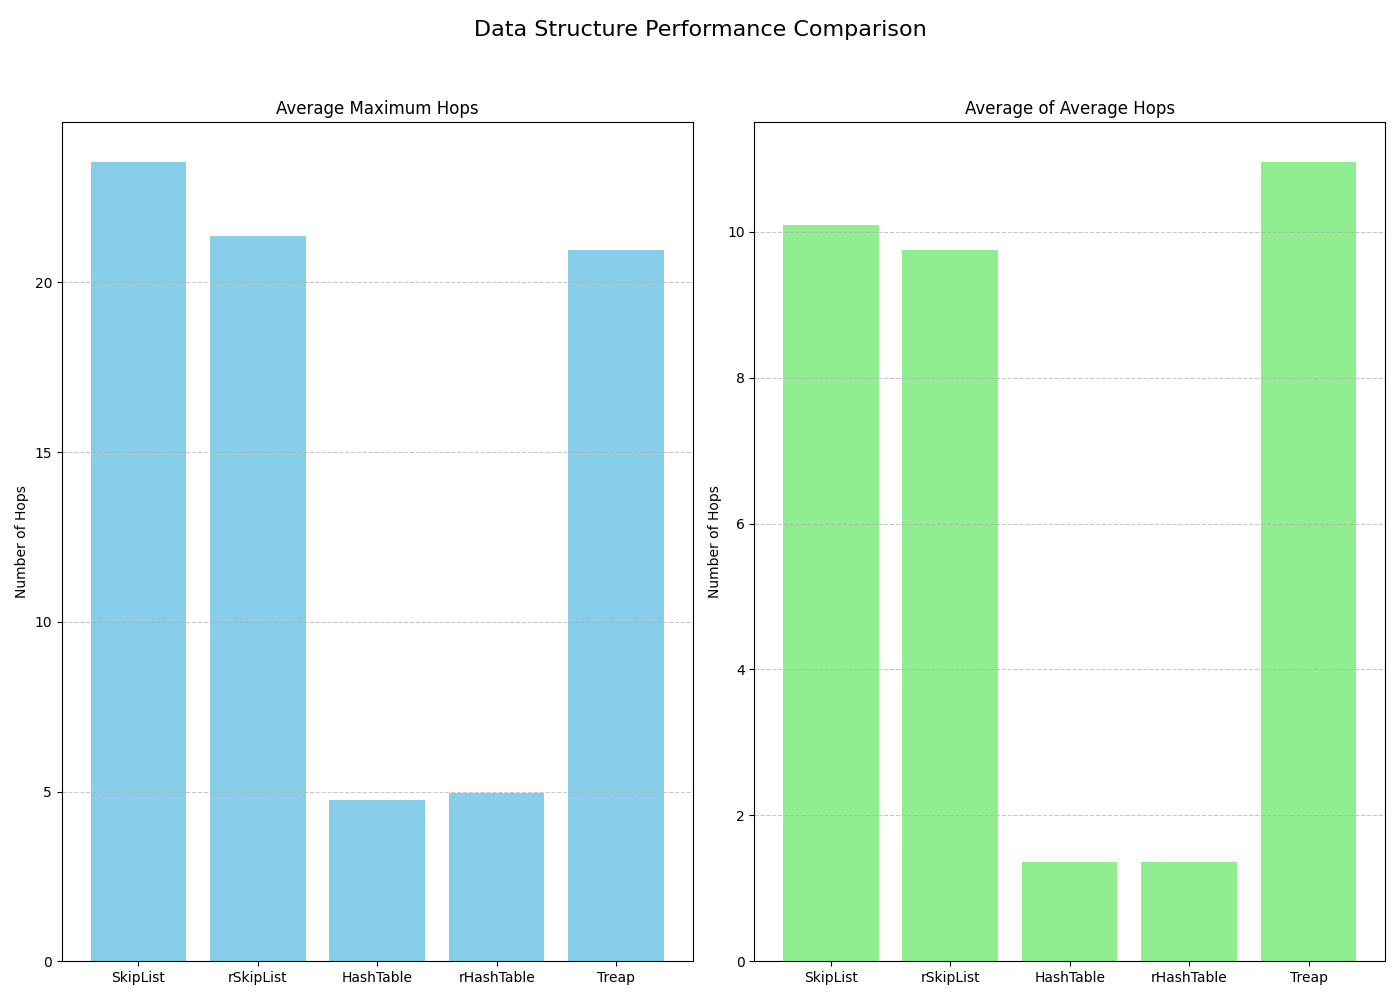
\includegraphics[width=\textwidth]{chapters/ch5_skipping/ch5_images/datastructure_performance.png}
    \caption[Non-adaptive PSDS Results.]{Maximum and average hop count in the non-adaptive setting, displayed on a linear scale.}
    \label{fig:runtimes_nonadaptive}
\end{figure}

\begin{figure}
    \centering
    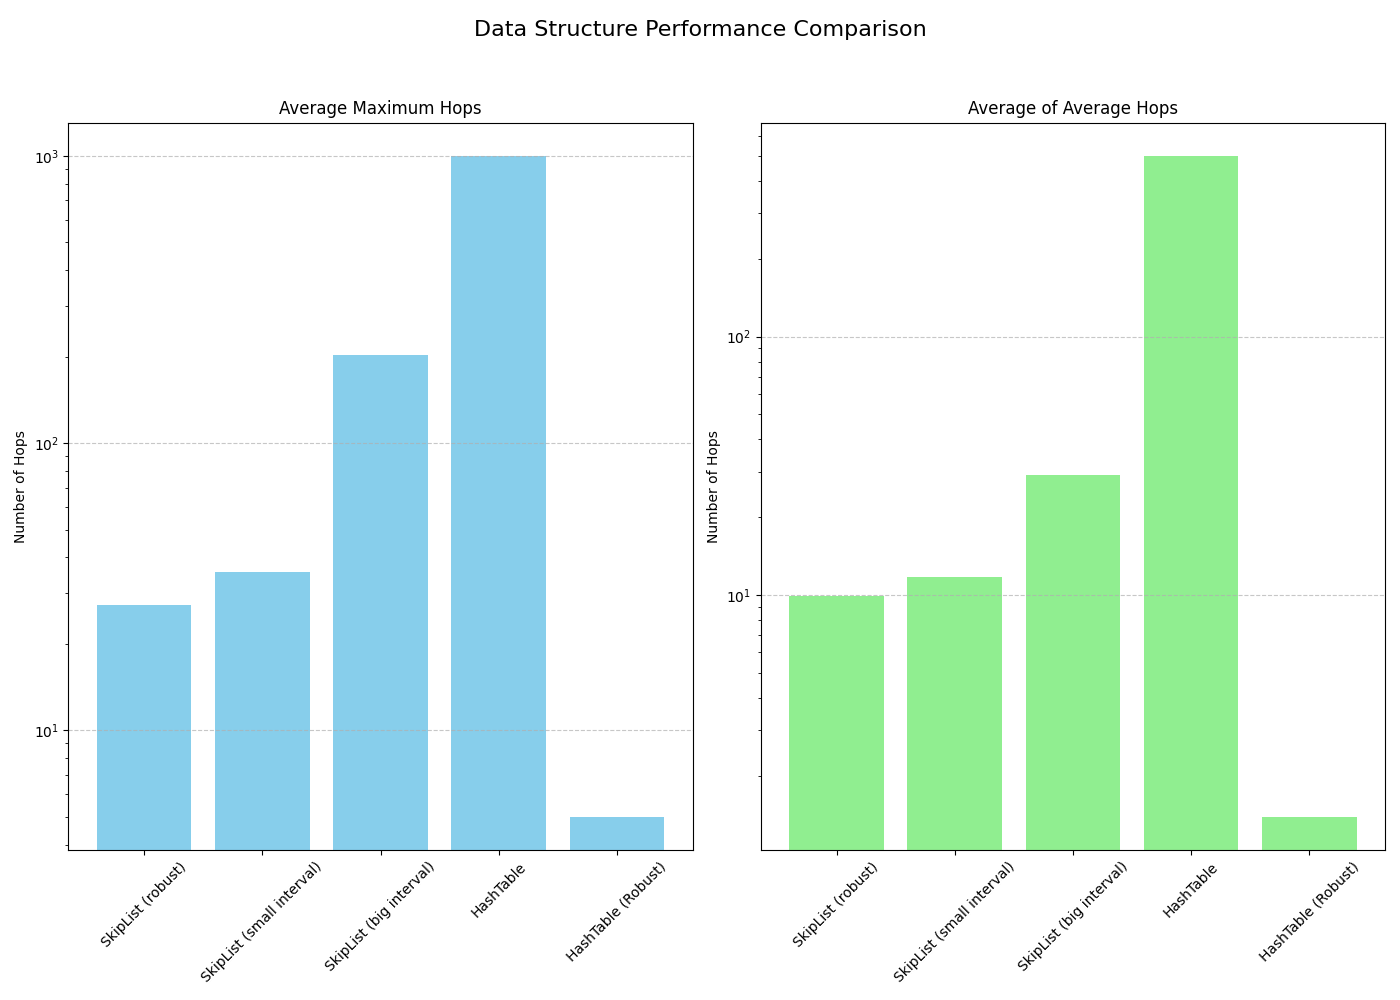
\includegraphics[width=\textwidth]{chapters/ch5_skipping/ch5_images/adaptive_datastructure_performance.png}
    \caption[Adaptive PSDS Results.]{Maximum and average hop count in the adaptive setting, displayed on a logarithmic scale.}
    \label{fig:runtimes_adaptive}
\end{figure}


We conducted experiments to empirically validate our analytical results. Our first experiment tested whether robust data structures offer benefits in non-adversarial settings. Using a dataset of 10 million usernames~\cite{10-mio}, we randomly inserted 1,000 usernames into each data structure. We measured performance by counting hops (forward movements between nodes). The hash table's load factor was limited to 0.7 \cite{mcclellan1974art}, and the skip list's maximum height was set to $log_{2} n$. We used Python's built-in hash function, which is vulnerable to multi-collision attacks. Results were averaged over 100 trials.

As shown in \Cref{fig:runtimes_nonadaptive}, the robust skip list consistently required fewer mean and maximum hops than its standard counterpart, demonstrating benefits even in non-adversarial settings with only constant overhead. The robust hash table showed comparable performance to the original structure. We benchmarked an unmodified treap implementation given its inherent adversarial robustness.

Our second experiment evaluated performance under adaptive adversarial conditions. We implemented a hash collision attack on hash tables and a gap attack on skip lists, averaging results over 100 trials. Treaps were excluded due to their established inherent robustness.

For the hash collision attack, we pre-calculated bucket values to deliberately insert all elements into a single bucket, creating worst-case conditions for standard hash tables. For the robust implementation, we used a random key for pre-calculation, since the actual secret key would be unknown to an attacker.

For the gap attack against skip lists, we tested two variants: a restricted version using the same username dataset and an unrestricted version using integers within the range $[0, 10^{100}]$\footnote{While this serves primarily as a proof of concept, such a vast interval could realistically be achieved using a 20-character limit with Unicode encoding. We emphasize that significant runtime degradation can be observed even with substantially smaller intervals.}. We report the top $1\%$ of outcomes with respect to the maximum hop count.

Results in~\Cref{fig:runtimes_adaptive} confirm that adversarial attacks significantly degrade standard implementations, while robust counterparts maintain consistent performance. The robust skip list maintained an average maximum hop count of 27.36, compared to 33.17 for the non-robust implementation under non-adaptive conditions. Under adaptive settings, the non-robust implementation degraded to 35.61 maximum average hops, and further to 202.71 hops when using the larger integer range. This validation confirms our theoretical findings on adversarial robustness, and also suggests that our remark regarding the artificial ``looseness'' of the bound carries weight.
%-------------------------------------------------------------------------------